\documentclass[10pt, UTF8]{book} %% ctexart

\title{\textbf{马克思主义基本原理}}
\author{钱锋\thanks{Email: strik0r.qf@gmail.com}${}^,$\thanks{
    西北工业大学软件学院, School of Software, Northwestern Polytechnical University, 西安 710072
}}

\usepackage{ctex}
\usepackage{graphicx}
\usepackage[toc]{multitoc}
\usepackage{booktabs}
\usepackage{longtable}
\usepackage{booktabs}
\usepackage{longtable}
\usepackage{amsthm, amssymb, amsmath, mathrsfs, mhchem}
\usepackage{tikz}
\usetikzlibrary{decorations.markings, angles, quotes}
\usepackage{pgfplots}
\usepackage{tikz-3dplot}
\usepackage{extpfeil}
\usepackage{diagbox}
\usepackage{float}
\usepackage{hyperref}
\hypersetup{hidelinks,
    colorlinks = true,
    allcolors = black,
    pdfstartview = Fit,
    breaklinks = true}
\usepackage{caption}
\usepackage{enumitem}
\usepackage{siunitx}
\usepackage{cuted}

\usepackage{titlesec} % 定义标题样式

% 设置 chapter 标题样式
\titleformat{\chapter}[hang]{\centering\heiti\Large\bfseries}{第\,\thechapter\,章}{1em}{}

% 定义 section 标题格式
\titleformat{\section}[hang]{\heiti\centering\large\bfseries}{\thesection}{1em}{}

% 定义 subsection 标题格式
\titleformat{\subsection}[hang]{\heiti\bfseries}{\textbf{\thesubsection}}{1em}{}

% 定义 subsubsection 标题格式
\setcounter{secnumdepth}{3}
\renewcommand\thesubsubsection{\arabic{subsubsection}.}
\titleformat{\subsubsection}[hang]{\kaishu}{\quad\quad\thesubsubsection\,\,}{0em}{}

\usepackage{fancyhdr} % 用于自定义页眉页脚


% 设置页眉页脚样式
\fancypagestyle{plain}{%
    \fancyhf{} % 清空页眉页脚
    \fancyhead[RO,LE]{·\thepage·} % 页眉显示页码, RO表示奇数页右侧, LE表示偶数页左侧
    \fancyhead[LO]{\nouppercase{\rightmark}} % 页眉显示小节标题, LO表示奇数页左侧
    \fancyhead[RE]{\nouppercase{\leftmark}} % 页眉显示章节标题, RE表示偶数页右侧
    \renewcommand{\headrulewidth}{0.4pt} % 设置页眉横线的宽度
    \renewcommand{\footrulewidth}{0pt} % 取消页脚横线
}

\renewcommand{\headrule}{\hrule width\textwidth height\headrulewidth\vskip-\headrulewidth}

% % 取消奇偶页的页眉偏移
% \fancyhfoffset[RO,LE]{0pt}

% % 取消奇偶页的页眉偏移
% \fancyhfoffset[RO,LE]{0pt}

% 定义取消页眉的命令
\newcommand{\cancelheader}{%
    \fancyhead{} % 清空页眉
    \renewcommand{\headrulewidth}{0pt} % 取消页眉横线
    \renewcommand{\footrulewidth}{0pt} % 设置页脚横线的宽度
}

\renewcommand{\chaptermark}[1]{\markboth{第 \thechapter 章 \hspace{1em} #1}{}}
\renewcommand{\sectionmark}[1]{\markright{\thesection \, #1}}

\usepackage[
    paperwidth=210mm,
    paperheight=297mm,
    top=40mm,
    bottom=31.8mm,
    left=25.4mm,
    right=25.4mm,
    footskip=15mm % 通过这里的值来调整页脚与正文内容的垂直距离
]{geometry}

\usepackage{mdframed}
\mdfsetup{
  linewidth=0.4pt,
  frametitlebackgroundcolor=white, % 或者 transparent
  frametitlefont=\heiti\bfseries,
  frametitleaboveskip=10pt,
  frametitlebelowskip=5pt,
  frametitlealignment=\raggedright % 新增此行
}

\usepackage{smartdiagram}
\usepackage{multirow}
\usepackage{tasks}

\begin{document}

\newtheoremstyle{mytheoremstyle}
    {1.5ex}                                         % Space above
    {1.5ex}                                         % Space below
    {}                                              % Font for body
    {}                                              % Indent amount
    {\bfseries}                                     % Font for head
    {}                                              % Punctuation after head
    {0.5em plus 0.2em minus 0.1em}                  % Space after head
    {\thmname{#1}\thmnumber{ #2}.\thmnote{ (#3).}}

\theoremstyle{mytheoremstyle} \newtheorem{example}{例}[section]
\theoremstyle{mytheoremstyle} \newtheorem{key}{核心要点}[section]

\theoremstyle{plain} \newtheorem{thm}{分析论述}

\newtheoremstyle{my3theoremstyle}
    {1.5ex}                                         % Space above
    {1.5ex}                                         % Space below
    {}                                              % Font for body
    {}                                              % Indent amount
    {\kaishu}                                       % Font for head
    {}                                              % Punctuation after head
    {0.5em plus 0.2em minus 0.1em}                  % Space after head
    {\thmname{#1}\thmnumber{ #2}.\thmnote{ (#3).}}

\theoremstyle{my3theoremstyle}
\newtheorem*{remark}{注}
\newtheorem*{sol}{答案要点}
\newtheorem*{cmt}{评注}

\pagestyle{empty}
\begin{titlepage}
    \thispagestyle{empty}
    \centering
        \vspace*{2cm}
        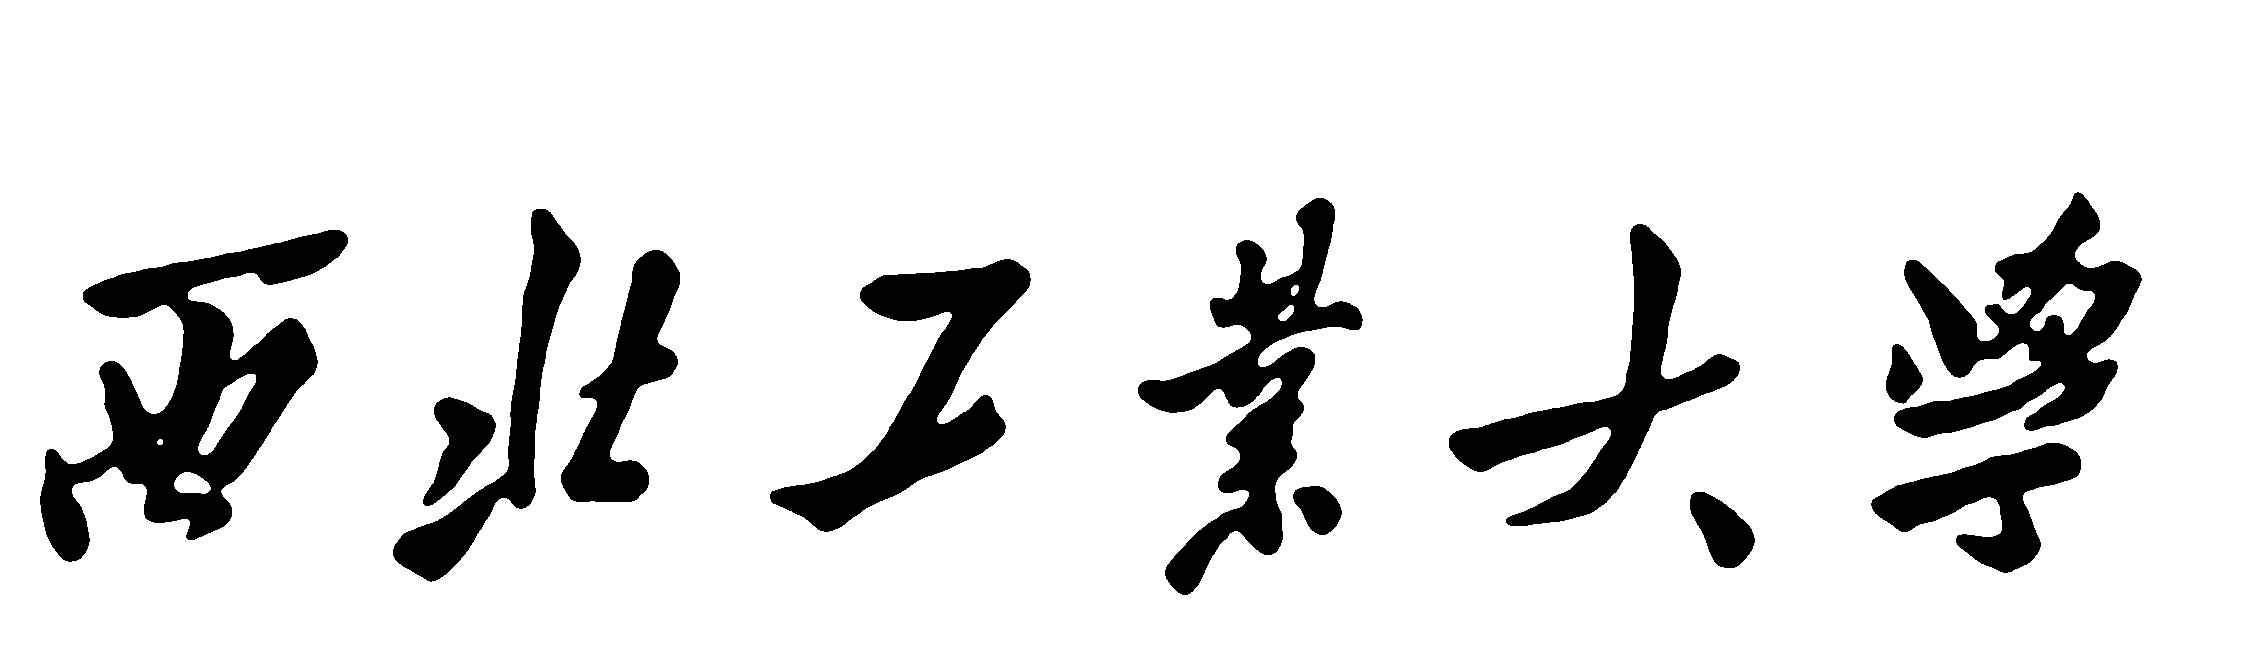
\includegraphics[width=0.5\textwidth]{pic/npu_2.png}\par
        \vspace{1em}
        
\includegraphics[width=0.5\textwidth]{pic/npu_1.png}\par
    \vspace{1em}
        \begin{center}
            \Huge \heiti \textbf{马克思主义基本原理}

            Fundamental Principles of Marxism
        \end{center}
        \vspace{16em}
        \begin{center}
        \songti
        \kaishu 数学与统计学院 \, \heiti\textbf{钱锋} \quad \songti 编
        \vspace{0.5em}

    \today
    \end{center}
\end{titlepage}

\cleardoublepage
\maketitle
\cleardoublepage

\frontmatter
\newpage
\pagestyle{plain}
\makeatother

% 设置目录页的页码格式
\pagenumbering{roman} % 切换回罗马数字页码
\addtocontents{toc}{\protect\thispagestyle{empty}}
\pagestyle{plain}
{\tableofcontents}
\newpage
\thispagestyle{empty}
\cleardoublepage % 确保正文从奇数页开始


% 设置章节标题页的页眉和页脚为空白页样式
\makeatletter
\let\ps@plain\ps@empty
\makeatother


\newpage
\chapter*{导 \quad 言}

\begin{quote}
    人类历史上不管在哪一个领域,包括创造财富的领域,做成大事业的绝非只有一些小伎俩的精明之人,
    而必是对世界和人生有广阔思考和独特领悟的拥有大智慧的人。
    
    真正的成功是做人的成功,即做一个有灵魂的人,一个精神上优秀的大写的人。这样的人即使在
    世俗的意义上不成功,他的人生仍是充满意义的。
    
    \begin{flushright}
        \kaishu —— 周国平
    \end{flushright}
\end{quote}

\newpage
\thispagestyle{empty}

\chapter{导论}

{\heiti\bfseries 复习建议:}
马克思主义基本原理课程中需要吸收运用的理论和概念很多,不适合突击速成,
全书共 97 个考点,在考研思想政治理论科目中占分 24\%,部分内容抽象且晦涩难懂,
是考研政治的重点、难点所在。建议准备期末考试的同学保证 60 天以上的复习时间,准备考研的
同学保证 180 天以上的复习时间。

\begin{table}[H]
    \small
    \centering
    \caption{《马克思主义基本原理》课程知识框架}
    \begin{tabular}{p{0.2\textwidth}|p{0.35\textwidth}|p{0.32\textwidth}}
        \hline
        \textbf{组成部分} & \textbf{章节内容} & \textbf{备注} \\
        \hline 
        导论 & 马克思主义是关于无产阶级和人类解放的科学 \\ 
        \hline
        \multirow{4}{0.2\textwidth}{马克思主义哲学} 
        & 辩证唯物论 & \multirow{4}{0.3\textwidth}{哲学部分占分 18/24,是马克思主义基本原理课程复习的重中之重。} \\
        & 唯物辩证法 & \\
        & 认识论 & \\
        & 唯物史观 & \\
        \hline 
        \multirow{2}{0.2\textwidth}{马克思主义政治经济学}
        & 资本主义的本质及规律 
        & \multirow{2}{0.3\textwidth}{西工大期末只考导论及前五章。} \\ 
        & 资本主义的发展及其趋势 & \\ 
        \hline 
        \multirow{2}{0.2\textwidth}{科学社会主义}
        & 社会主义的发展及其规律 & \\ 
        & 共产主义崇高理想及其最终实现 & \\ 
        \hline
    \end{tabular}
\end{table}

在人类思想史上,就科学性和影响力而言,没有一种思想理论能达到马克思主义的高度,
也没有一种学说能像马克思主义那样对世界产生如此广泛而深远的影响。这充分体现了马克思主义
的真理伟力,表明了马克思主义对人们认识世界、改造世界具有不可替代的作用。

\section{马克思主义的创立和发展}

\subsection{马克思主义的内涵及其构成}

\subsubsection{马克思主义的内涵}

马克思主义(Marxism)是由马克思\footnote{
    马克思(Karl Marx)是19世纪德国哲学家、经济学家、社会学家和革命家,被视为现代社会科学的奠基人之一。他的著作《资本论》等著名著作探讨了资本主义经济的运作机制和阶级斗争的规律,提出了无产阶级革命的理论,并呼吁建立一个没有私有制的社会主义社会。
}和恩格斯\footnote{
    恩格斯(Friedrich Engels)是马克思的朋友、合作者和理论继承者,也是19世纪德国的哲学家、社会科学家和革命家。他与马克思合著了《共产党宣言》等重要文献,深入研究了资本主义的发展和工人阶级的境遇,为马克思主义理论的发展作出了重要贡献,也积极参与了国际工人运动。
}创立并为后继者所不断发展的科学理论体系(起源与发展),
是关于自然、社会和人类思维发展的一般规律的学说(内容、马克思主义哲学),是关于社会主义必然代替资本主义、
最终实现共产主义的学说(目的、马克思主义政治经济学),
是关于无产阶级解放、全人类解放和每个人自由而全面发展的学说(立场,科学社会主义),
是无产阶级政党和社会主义国家的指导思想,是指引人民创造美好生活的行动指南(意义)。
\begin{remark}
    马克思主义的内涵,可以从六个角度来划分理解,这些划分的角度就是上文中括号中的内容。
    马克思主义的内涵在考试中一般不做考察,但近两年的考研政治出题越来越出其不意,还是
    尽量了解一下。
\end{remark}

\subsubsection{马克思主义的构成}



马克思主义是一个博大精深的理论体系。恩格斯在《反杜林论》({\itshape Anti-Dühring})\footnote{
    《反杜林论》是由恩格斯撰写的重要文献,旨在批判德国哲学家杜林的唯心主义哲学观点。
    该文指出了杜林在对待自然科学和历史发展等问题上的错误观点,强调了历史唯物主义的重要性,
    并阐述了历史唯物主义对社会发展和阶级斗争的解释。
    恩格斯在《反杜林论》中提出了马克思主义唯物史观的基本原理,
    \textbf{首次将马克思主义以三个组成部分的形式进行了全面阐述},
    为马克思主义思想的发展做出了重要贡献。
}一文中将马克思主义的理论分成了
三个基本组成部分:
\begin{itemize}[itemsep=0pt]
    \item 研究的基本理论和方法:马克思主义\textbf{哲学}(Marxist Philosophy);
    \item 主体内容:马克思主义\textbf{政治经济学}(Marxist Political Economy);
    \item 目的与归宿:\textbf{科学社会主义}(Scientific Socialism)。
\end{itemize}
% 这三个基本组成部分有机统一并共同构成了马克思主义理论的主体内容。
从这一层面上来讲,马克思主义是以马克思主义政治经济学为主体内容的,以马克思主义哲学作为
研究的基本理论与基本方法的,以科学社会主义作为最终目的与最终归宿的理论体系。
\begin{figure}[H]
    \centering
    

\tikzset{every picture/.style={line width=0.75pt}} %set default line width to 0.75pt        

\begin{tikzpicture}[x=0.75pt,y=0.75pt,yscale=-0.9,xscale=0.9]
%uncomment if require: \path (0,300); %set diagram left start at 0, and has height of 300

%Straight Lines [id:da7900404923689658] 
\draw  [dash pattern={on 0.84pt off 2.51pt}]  (354,55.5) -- (434,55.5) ;
%Straight Lines [id:da2776322276809655] 
\draw  [dash pattern={on 0.84pt off 2.51pt}]  (399,126.5) -- (435,126.5) ;
%Straight Lines [id:da8162475035000624] 
\draw  [dash pattern={on 0.84pt off 2.51pt}]  (400,194.5) -- (436,194.5) ;
%Straight Lines [id:da9764304210153608] 
\draw    (291,73.5) -- (291,105.5) ;
\draw [shift={(291,107.5)}, rotate = 270] [color={rgb, 255:red, 0; green, 0; blue, 0 }  ][line width=0.75]    (10.93,-3.29) .. controls (6.95,-1.4) and (3.31,-0.3) .. (0,0) .. controls (3.31,0.3) and (6.95,1.4) .. (10.93,3.29)   ;
%Straight Lines [id:da2506247619262363] 
\draw    (291,141.5) -- (291,173.5) ;
\draw [shift={(291,175.5)}, rotate = 270] [color={rgb, 255:red, 0; green, 0; blue, 0 }  ][line width=0.75]    (10.93,-3.29) .. controls (6.95,-1.4) and (3.31,-0.3) .. (0,0) .. controls (3.31,0.3) and (6.95,1.4) .. (10.93,3.29)   ;
%Straight Lines [id:da3783928279477312] 
\draw  [dash pattern={on 0.84pt off 2.51pt}]  (291,210.5) -- (291,244.5) ;
%Shape: Brace [id:dp8337992157264561] 
\draw   (225,56.5) .. controls (220.33,56.5) and (218,58.83) .. (218,63.5) -- (218,115) .. controls (218,121.67) and (215.67,125) .. (211,125) .. controls (215.67,125) and (218,128.33) .. (218,135)(218,132) -- (218,186.5) .. controls (218,191.17) and (220.33,193.5) .. (225,193.5) ;

% Text Node
\draw (162,126) node   [align=left] {\begin{minipage}[lt]{68pt}\setlength\topsep{0pt}
马克思主义的\\三大组成部分
\end{minipage}};
% Text Node
\draw (290.5,56.75) node   [align=left] {\begin{minipage}[lt]{83.64pt}\setlength\topsep{0pt}
马克思主义哲学
\end{minipage}};
% Text Node
\draw (312.5,124.75) node   [align=left] {\begin{minipage}[lt]{113.56pt}\setlength\topsep{0pt}
马克思主义政治经济学
\end{minipage}};
% Text Node
\draw (313.5,193.75) node   [align=left] {\begin{minipage}[lt]{113.56pt}\setlength\topsep{0pt}
科学社会主义
\end{minipage}};
% Text Node
\draw (487,56) node   [align=left] {\begin{minipage}[lt]{69.36pt}\setlength\topsep{0pt}
德国古典哲学
\end{minipage}};
% Text Node
\draw (508.5,126) node   [align=left] {\begin{minipage}[lt]{98.6pt}\setlength\topsep{0pt}
英国古典政治经济学
\end{minipage}};
% Text Node
\draw (502,194) node   [align=left] {\begin{minipage}[lt]{88.4pt}\setlength\topsep{0pt}
英法空想社会主义
\end{minipage}};
% Text Node
\draw (297,81) node [anchor=north west][inner sep=0.75pt]   [align=left] {作为思想和方法};
% Text Node
\draw (297,149) node [anchor=north west][inner sep=0.75pt]   [align=left] {作为理论依据};
% Text Node
\draw (250,250) node [anchor=north west][inner sep=0.75pt]   [align=left] {最终的目的与归宿};


\end{tikzpicture}
\caption{马克思主义的三大组成部分}
\end{figure}


\subsection{马克思主义的基本立场、基本观点和基本方法}

马克思主义基本原理是对马克思主义立场、观点、方法的集中概括,是马克思主义在其形成、
发展和运用过程中经过时间反复检验而确立起来的具有普遍真理性的理论。它体现马克思主义的
根本性质和整体特征,体现马克思主义科学性和革命性的统一。相对于特定历史条件下
所做的个别理论判断和具体结论,马克思主义基本原理具有普遍的、根本的和长远的指导意义。

我们可以从基本立场、基本观点、基本方法的有机统一中,来学习和把握马克思主义。

\subsubsection{马克思主义的基本立场}

马克思主义的基本立场,是马克思主义观察、分析和解决问题的根本立足点和出发点。
\textbf{马克思主义以无产阶级的解放和全人类的解放为己任,以人的自由全面发展为美好目标,以人民为中心,
一切为了人民,一切依靠人民,全心全意为人民服务。}

\subsubsection{马克思主义的基本观点}

马克思主义的基本观点,是关于自然、社会和人类思维发展一般规律的科学认识,是对人类思想成果和
社会实践经验的科学总结。这些基本观点主要包括:
\begin{tasks}(2)
    \task 关于世界统一于物质、物质决定意识的观点;
    \task 关于事物矛盾运动规律的观点;
    \task 关于实践和认识辩证关系的观点;
    \task 关于社会存在决定社会意识的观点;
    \task 关于人与自然和谐共生的观点;
    \task 关于人类社会基本矛盾运动规律的观点;
    \task 关于人的自由而全面发展的观点;
    \task 关于世界历史的观点;
    \task 关于阶级和阶级斗争的观点;
    \task 关于人民群众创造历史的观点;
    \task 关于劳动价值论的观点;
    \task 关于剩余价值和资本主义生产方式本质的观点;
    \task 关于资本主义政治制度和意识形态本质的观点;
    \task 关于垄断资本主义的观点;
    \task 关于社会主义必然代替资本主义的观点;
    \task 关于社会主义革命和无产阶级专政的观点;
    \task 关于无产阶级政党建设的观点;
    \task 关于社会主义社会本质特征和建设规律的特点;
    \task 关于共产主义社会基本特征和共产主义远大理想的观点;
    \task ……
\end{tasks}
\begin{remark}
    “科学性是马克思主义独有的特点”,这一表述在思想政治类课程学习和考研政治中是一个
    基本的论调。
\end{remark}
\begin{remark}
    从内容的角度来分析马克思主义的内涵,是说{\kaishu 马克思主义是关于自然、社会和人类思维发展的
    一般规律的学说},这两个知识点可以结合在一起记忆。马克思主义的内容是关于自然、社会和人类思维发
    展一般规律的,所以它的基本观点就是关于自然、社会和人类思维发展的一般规律的科学认识。
\end{remark}

\subsubsection{马克思主义的基本方法}

马克思主义的基本方法,是建立在辩证唯物主义和历史唯物主义世界观和方法论基础上,
指导我们正确认识世界和改造世界的思想方法和工作方法。它们包括:
\begin{tasks}(2)
    \task 实事求是的方法;
    \task 辩证分析的方法;
    \task 社会基本矛盾和主要矛盾分析的方法;
    \task 历史分析的方法;
    \task 阶级分析的方法;
    \task 群众路线的方法
    \task ……
\end{tasks}

\subsection{马克思主义的创立}



\subsubsection{马克思主义创立的社会根源、阶级基础和思想渊源}

马克思主义产生于 19 世纪 40 年代,创始人是马克思和恩格斯。
马克思主义的产生具有深刻的社会根源、阶级基础和思想渊源。
\begin{itemize}[itemsep=0pt]
    \item 社会根源:\textbf{资本主义生产方式在欧洲已经有了相当的发展}:
    {\small 工业革命和科技进步极大地提高了劳动生产率,促进了生产力的发展。
    资本主义生产方式一方面带来了社会化大生产的迅猛发展,另一方面又造成了
    深重的社会灾难:
    \begin{enumerate}[itemsep=0pt, label=$\left.\arabic*\right)$]
        \item 社会两极分化,工人极端困苦。机器大工业的发展,不仅没有改善工人的劳动和
        生活条件,而且使工人成为机器的附庸。资本家采取延长劳动时间、增大劳动强度、
        降低工人工资、廉价雇佣女工和童工等手段,拼命压榨工人血汗,无产阶级与资产阶级
        的矛盾不断加剧。
        \item 周期性经济危机频繁爆发。英国在工业革命开始后,曾多次发生局部性经济危机,
        每一次经济危机都对社会造成巨大的破坏。
    \end{enumerate}}
    \item 阶级基础:无产阶级在反抗资产阶级剥削和压迫斗争的斗争中,逐渐走向自觉,并迫切
    渴望科学的理论指导,法国、英国、德国工人运动的兴起,标志着现代无产阶级作为独立的
    政治力量登上了历史舞台。\textbf{觉醒了的无产阶级迫切需要总结和升华自身的斗争经验,
    形成科学的革命理论,以指导自身的解放斗争}。
    \item 思想渊源:
    \begin{figure}[H]
        \centering
    
    
    \tikzset{every picture/.style={line width=0.75pt}} %set default line width to 0.75pt        
    
    \begin{tikzpicture}[x=0.75pt,y=0.75pt,yscale=-1,xscale=1]
    %uncomment if require: \path (0,449); %set diagram left start at 0, and has height of 449
    
    %Shape: Brace [id:dp8589737925705583] 
    \draw   (244,72.5) .. controls (239.33,72.5) and (237,74.83) .. (237,79.5) -- (237,172) .. controls (237,178.67) and (234.67,182) .. (230,182) .. controls (234.67,182) and (237,185.33) .. (237,192)(237,189) -- (237,284.5) .. controls (237,289.17) and (239.33,291.5) .. (244,291.5) ;
    %Shape: Brace [id:dp8773220460912701] 
    \draw   (364,27.5) .. controls (359.33,27.5) and (357,29.83) .. (357,34.5) -- (357,63.75) .. controls (357,70.42) and (354.67,73.75) .. (350,73.75) .. controls (354.67,73.75) and (357,77.08) .. (357,83.75)(357,80.75) -- (357,113) .. controls (357,117.67) and (359.33,120) .. (364,120) ;
    %Shape: Brace [id:dp6324604138620569] 
    \draw   (365,153.5) .. controls (360.33,153.5) and (358,155.83) .. (358,160.5) -- (358,189.75) .. controls (358,196.42) and (355.67,199.75) .. (351,199.75) .. controls (355.67,199.75) and (358,203.08) .. (358,209.75)(358,206.75) -- (358,239) .. controls (358,243.67) and (360.33,246) .. (365,246) ;
    
    % Text Node
    \draw (142,162) node [anchor=north west][inner sep=0.75pt]   [align=left] {马克思主义\\的思想渊源};
    % Text Node
    \draw (252,64) node [anchor=north west][inner sep=0.75pt]   [align=left] {直接理论来源};
    % Text Node
    \draw (372,26) node [anchor=north west][inner sep=0.75pt]   [align=left] {德国古典哲学};
    % Text Node
    \draw (372,65) node [anchor=north west][inner sep=0.75pt]   [align=left] {英国古典政治经济学};
    % Text Node
    \draw (372,103) node [anchor=north west][inner sep=0.75pt]   [align=left] {英法空想社会主义};
    % Text Node
    \draw (252,192) node [anchor=north west][inner sep=0.75pt]   [align=left] {自然科学前提};
    % Text Node
    \draw (372,149) node [anchor=north west][inner sep=0.75pt]   [align=left] {细胞学说};
    % Text Node
    \draw (372,194) node [anchor=north west][inner sep=0.75pt]   [align=left] {能量守恒与转化定律};
    % Text Node
    \draw (372,230) node [anchor=north west][inner sep=0.75pt]   [align=left] {生物进化论};
    % Text Node
    \draw (252,273) node [anchor=north west][inner sep=0.75pt]   [align=left] {其他思想来源};
    
    
    \end{tikzpicture}
    \caption{马克思主义的思想渊源}
    \end{figure}
    \begin{enumerate}[itemsep=0pt, label=$\left.\arabic*\right)$]
        \item 19 世纪西欧三大先进思潮为马克思主义的创立提供了直接的理论来源。
            \begin{itemize}[itemsep=0pt]
                \item \textbf{德国古典哲学} (classical philosophy):
                辩证法思想;
                \item \textbf{英国古典政治经济学} (classical political economy):对资本主义生产关系的分析和关于
                劳动创造价值的思想;
                \item \textbf{英法空想社会主义} 
                (Utopian socialism):
                对资本主义社会的批判和对未来新社会的展望,
            \end{itemize}
            这三大思潮都是资本主义发展初期的先进的思想家求索时代课题的尝试。
    
        \item 19 世纪的三大科学发现,即\textbf{细胞学说}、
        \textbf{能量守恒与转化定律}、\textbf{生物进化论},为马克思主义的产生提供了自然科学前提。

        \item 从更广泛的意义上讲,马克思主义的思想来源还有古希腊、罗马哲学、文艺复兴运动的思想成果、
        法国复辟时期历史学家的进步思想等。
    \end{enumerate}
\end{itemize}



\subsubsection{马克思与恩格斯的早期经历与世界观和政治立场的彻底转变}

从优越的家庭条件和卓越的个人才华来说,马克思和恩格斯完全有可能跻身所谓的 “上流社会”,
求得令人羡慕的个人前程,但是他们放弃了舒适安逸的生活,毅然选择了充满荆棘与坎坷的革命
之路。

马克思和恩格斯发表在 1844 年 2 月《德法年鉴》上的论文表明,他们完成了从唯心主义向
唯物主义、从革命民主主义向共产主义的转变(称为 “两个转变”),
为创立马克思主义奠定了思想前提。

\subsubsection{《共产党宣言》的发表和马克思主义的公开问世}

马克思、恩格斯接受国际性工人组织 “正义者同盟” 的邀请,将其改组为 \textbf{“共产主义者同盟”,
这是世界上第一个共产主义政党}。并为其起草了\textbf{世界上第一个无产阶级政党的党纲
——《共产党宣言》}。1848 年 2 月,\textbf{《共产党宣言》发表,标志着马克思主义的公开问世,
标志着科学社会主义的诞生,标志着马克思主义的诞生}。
\begin{remark}
    这里需要注意的是,组织并不等于政党。因此 “正义者同盟” 仅仅是一个国际性的工人组织,
    而不是共产主义政党。世界上的第一个共产主义政党是 “无产主义者同盟”。这两个组织的
    名字里都带有 “同盟”,却具有完全不同的性质,前者是一个工人组织,而后者则是一个无产阶级政党。
\end{remark}

\subsubsection{总结革命经验 \quad 丰富革命理论}

1848 年欧洲革命失败后,他们流亡英国。马克思进行了全面深入的政治经济学研究,撰写了《资本论》
并出版了第一卷,系统阐述了剩余价值学说,揭示了资本主义生产关系的秘密。
\textbf{唯物史观和剩余价值学说是马克思一生的两个伟大发现}。

% \begin{table}[H]
%     \centering
%     \caption{马克思与恩格斯的经典著作}
%     \begin{tabular}{p{0.2\textwidth}|p{0.3\textwidth}p{0.2\textwidth}p{0.2\textwidth}}
%         \hline
%         \textbf{作品} & \textbf{内容} & \textbf{关键词} & \textbf{备注} \\
%         \hline
%         《德法年鉴》(期刊)
%         \newline 马克思、恩格斯 \newline 1844.2
%         & 马克思、恩格斯在《德法年鉴》上分别发表了两篇文章,标志着马克思和恩格斯的两个转变,
%         即从唯心主义转向唯物主义、从革命民主主义转向共产主义,这为马克思、恩格斯创立自己的理论奠定了
%         思想前提
%         & 两个转变 \\ 
%         \hline
%         《德意志意识形态》
%         \newline 马克思、恩格斯 
%         & 首次系统阐了历史唯物主义的基本观点,实现了历史观上的伟大变革,
%         标志着马克思主义哲学的诞生
%         & 唯物史观的创立 \newline 马克思主义哲学的诞生 \\ 
%         \hline 
%         《共产党宣言》
%         \newline 马克思、恩格斯 \newline 1848.2
%         & 标志着科学社会主义、马克思主义的诞生,是世界上第一个无产阶级政党的党纲
%         & 科学社会主义的诞生 \newline 马克思主义的诞生 \newline 首个无产阶级政党党纲 \\
%         \hline 
%         《资本论》
%         \newline 马克思 
%         & 系统阐述剩余价值理论,标志着马克思主义政治经济学的诞生
%         & 政治经济学的诞生 & 被称为 “工人阶级的圣经” \\ 
%         \hline 
%         《反杜林论》
%         \newline 恩格斯 
%         & 首次将马克思主义以三个组成部分(马克思主义哲学、政治经济学、科学社会主义)
%         的形式进行了全面阐述
%         & 全面阐述 \newline 三个组成部分
%         & 被称为 “马克思主义的百科全书” \\
%         \hline
        
%         《关于费尔巴哈的提纲》 \newline 马克思 
%         & 首次确立了科学的实践观 
%         & 实践观 \newline 历史唯物主义的起源 \\
%         \hline
%         《家庭、私有制和国家的起源》 \newline 恩格斯 
%         & 关于古代社会发展规律的著作,是马克思主义国家学说的代表作之一 
%         & 国家学说 \\ 
%         \hline
%     \end{tabular}
% \end{table}

{\small 
\begin{longtable}{p{0.2\textwidth}|p{0.3\textwidth}p{0.15\textwidth}p{0.2\textwidth}}
    \caption{马克思与恩格斯的经典著作}\\
    \hline
    \textbf{作品} & \textbf{内容} & \textbf{关键词} & \textbf{备注} \\
    \hline
    \endfirsthead
    
    \multicolumn{4}{r}%
    {(续表)} \\
    \hline
    \textbf{作品} & \textbf{内容} & \textbf{关键词} & \textbf{备注} \\
    \hline
    \endhead
    
    \hline \multicolumn{4}{r}{{续下页}} \\
    \endfoot
    
    \hline
    \endlastfoot
    
    《德法年鉴》(期刊)
    
    马克思、恩格斯
    
    1844.2
    & 马克思、恩格斯在《德法年鉴》上分别发表了两篇文章,标志着马克思和恩格斯的两个转变,
    即从唯心主义转向唯物主义、从革命民主主义转向共产主义,这为马克思、恩格斯创立自己的理论奠定了
    思想前提
    & 两个转变 \\ 
    \hline
    《德意志意识形态》
    \newline 马克思、恩格斯 
    & 首次系统阐了历史唯物主义的基本观点,实现了历史观上的伟大变革,
    标志着马克思主义哲学的诞生
    & 唯物史观的创立 \newline 马克思主义哲学的诞生 \\ 
    \hline 
    《共产党宣言》
    \newline 马克思、恩格斯 \newline 1848.2
    & 标志着科学社会主义、马克思主义的诞生,是世界上第一个无产阶级政党的党纲
    & 科学社会主义的诞生 \newline 马克思主义的诞生 \newline 首个无产阶级政党党纲 \\
    \hline 
    《资本论》
    \newline 马克思 
    & 系统阐述剩余价值理论,标志着马克思主义政治经济学的诞生
    & 政治经济学的诞生 & 被称为 “工人阶级的圣经” \\ 
    \hline 
    《反杜林论》
    \newline 恩格斯 
    & 首次将马克思主义以三个组成部分(马克思主义哲学、政治经济学、科学社会主义)
    的形式进行了全面阐述
    & 全面阐述 \newline 三个组成部分
    & 被称为 “马克思主义的百科全书” \\
    \hline
    
    《关于费尔巴哈\footnote{
        费尔巴哈(Ludwig Feuerbach)是19世纪德国哲学家,代表作有《基督教的本质》。他对黑格尔哲学进行批判,认为宗教是人类自身本质的投射,主张将神的属性还归给人类自身,以实现人的解放与自我意识觉醒。他的思想强调了人本身的重要性,为后来的唯物主义和人本主义哲学奠定了重要基础。
    }的提纲》 \newline 马克思 
    & 首次确立了科学的实践观 
    & 实践观 \newline 历史唯物主义的起源 \\
    \hline
    《家庭、私有制和国家的起源》 \newline 恩格斯 
    & 关于古代社会发展规律的著作,是马克思主义国家学说的代表作之一 
    & 国家学说 \\ 
    \hline
\end{longtable}}

\subsection{马克思主义的发展}

列宁深刻分析了 19 世纪末 20 世纪初世界历史条件的变化,认为随着资本主义发展到
垄断阶段,经济政治发展的不平衡已成为资本主义发展的绝对规律,提出了社会主义革命可能在
一国或数国首先发生并取得胜利的论断。
\begin{remark}
    注意这里的因果关系,经济政治发展的不平衡是因,而社会主义革命可能会发生和胜利则是结果。
\end{remark}




\section{马克思主义的鲜明特征和当代价值}

\subsection{马克思主义的鲜明特征}

马克思主义具有鲜明的科学性、人民性、实践性、发展性,这些特征体现了马克思主义的
本质和使命,也展现出马克思主义的理论形象。
\begin{itemize}[itemsep=0pt]
    \item \textbf{科学性}:马克思主义是对自然、社会和人类思维发展本质和规律的正确反映;
    \item \textbf{人民性}:\textbf{人民至上是马克思主义的政治立场};
    \item \textbf{实践性}:从实践中来、到实践中去、在实践中接受检验、随实践而不断发展;
    \item \textbf{发展性}:不断发展、与时俱进。
\end{itemize}
马克思主义的人民性、实践性和发展性,集中表现为革命性。因此,马克思主义的鲜明特征,
如果用一句话来概括,就是\textbf{科学性与革命性的统一}。

\begin{figure}[H]
    \centering
    

\tikzset{every picture/.style={line width=0.75pt}} %set default line width to 0.75pt        

\begin{tikzpicture}[x=0.75pt,y=0.75pt,yscale=-1,xscale=1]
%uncomment if require: \path (0,300); %set diagram left start at 0, and has height of 300

%Shape: Rectangle [id:dp5743918056710222] 
\draw  [dash pattern={on 1.69pt off 2.76pt}][line width=1.5]  (135,99) -- (402,99) -- (402,187.5) -- (135,187.5) -- cycle ;

% Text Node
\draw    (68,111.75) -- (125,111.75) -- (125,143.75) -- (68,143.75) -- cycle  ;
\draw (96.5,127.75) node   [align=left] {\begin{minipage}[lt]{36.04pt}\setlength\topsep{0pt}
科学性
\end{minipage}};
% Text Node
\draw    (154,111.75) -- (211,111.75) -- (211,143.75) -- (154,143.75) -- cycle  ;
\draw (182.5,127.75) node   [align=left] {\begin{minipage}[lt]{36.04pt}\setlength\topsep{0pt}
人民性
\end{minipage}};
% Text Node
\draw    (240,111.75) -- (297,111.75) -- (297,143.75) -- (240,143.75) -- cycle  ;
\draw (268.5,127.75) node   [align=left] {\begin{minipage}[lt]{36.04pt}\setlength\topsep{0pt}
实践性
\end{minipage}};
% Text Node
\draw    (326,111.75) -- (383,111.75) -- (383,143.75) -- (326,143.75) -- cycle  ;
\draw (354.5,127.75) node   [align=left] {\begin{minipage}[lt]{36.04pt}\setlength\topsep{0pt}
发展性
\end{minipage}};
% Text Node
\draw (245,162) node [anchor=north west][inner sep=0.75pt]   [align=left] {革命性};


\end{tikzpicture}
\caption{马克思主义的鲜明特征}
\end{figure}

\subsection{马克思主义的当代价值}

\subsubsection{观察当代世界变化的认识工具}
马克思主义给予我们观察当代世界的宏大视野,给予我们透视时代风云的锐利目光,
给予我们展望未来世界的长远眼光和战略定力。
\subsubsection{指引当代中国发展的行动指南}
马克思主义是指引当代中国发展的精神旗帜,是推动当代中国发展的精神动力,
是引领当代中国实践的行动指南。
\subsubsection{引领人类社会进步的科学真理}
社会是在矛盾中进步的,每一个时代的社会进步总是伴随着相应的
社会问题,人类社会怎样面对和处理这些问题,怎样才能走向更加美好的明天?
回答和解决这样的根本性问题,还是需要到马克思主义中寻找智慧。

\vspace*{1em}
大学生在学习马克思主义的过程中,要有正确的学习态度和科学的学习方法。
第一,要努力学习和掌握马克思主义的基本立场、观点、方法;
第二,要努力学习和掌握马克思主义中国化的理论成果;
第三,要坚持理论联系实际的马克思主义学风;
第四,要自觉将马克思主义内化于心,外化于行。

\clearpage
\thispagestyle{empty}
\mainmatter

\part{马克思主义哲学}

\chapter{世界的物质性及发展规律}

% \begin{tasks}(2)
%     \task 辩证唯物主义物质范畴
%     \task 世界的物质统一性
%     \task 主观能动性与客观规律性的辩证统一
%     \task 联系和发展的基本规律
%     \task 唯物辩证法是科学的认识方法
%     \task 在实践中不断增强思维能力
% \end{tasks}

% 客观实在性是物质的共同特性,是指存在于人的意识之外,不以人的意志为转移并能为
% 人所感知的客观存在,即物质世界。不管物质的形态、结构和属性如何千变万化,其客观实在
% 的属性在任何时候、任何地方都是不变的,因而具有永恒性和绝对性,客观实在性是万事万物
% 共有的特性。

% 意识的内容是客观的,而在形式上是主观的,所以意识是客观内容和主观形式的统一。

% 相对于过去的运动到达一个变化点或者一个转折点,该点即静止,也为结果,从这点开始了一个新的运动,
% 即新运动的出发点。



% \section{哲学及其基本问题}

\section{世界的多样性与物质统一性}

\subsection{物质及其存在方式}

% \subsection{哲学是系统化、理论化的世界观}

哲学是系统化、理论化的世界观,是对自然知识、社会知识和思维知识的概括和总结,
哲学世界观起源于人类在生活实践中对世界的追问和思考,
是关于宇宙和人生的总体性认识,为人类安身立命提供不可或缺的思想基础。

\begin{figure}[H]
    \centering


\tikzset{every picture/.style={line width=0.75pt}} %set default line width to 0.75pt        

\begin{tikzpicture}[x=0.75pt,y=0.75pt,yscale=-1,xscale=1]
%uncomment if require: \path (0,300); %set diagram left start at 0, and has height of 300

%Straight Lines [id:da06915972307109763] 
\draw    (308,110.5) -- (308,150.5) ;
\draw [shift={(308,153.5)}, rotate = 270] [fill={rgb, 255:red, 0; green, 0; blue, 0 }  ][line width=0.08]  [draw opacity=0] (6.25,-3) -- (0,0) -- (6.25,3) -- cycle    ;

% Text Node
\draw (174,81) node [anchor=north west][inner sep=0.75pt]   [align=left] {世界观:人们对世界的总的看法和根本观点};
% Text Node
\draw (174,166) node [anchor=north west][inner sep=0.75pt]   [align=left] {方法论:人们认识世界和改造世界的根本原则和根本方法};
% Text Node
\draw (319,121) node [anchor=north west][inner sep=0.75pt]   [align=left] {决定};


\end{tikzpicture}
\caption{世界观与方法论}
\end{figure}

\begin{figure}[H]
    \centering
    



    \tikzset{every picture/.style={line width=0.75pt}} %set default line width to 0.75pt        

    \begin{tikzpicture}[x=0.75pt,y=0.75pt,yscale=-1,xscale=1]
    %uncomment if require: \path (0,300); %set diagram left start at 0, and has height of 300
    
    %Shape: Brace [id:dp1198995538704497] 
    \draw   (236,73.5) .. controls (231.33,73.5) and (229,75.83) .. (229,80.5) -- (229,111.25) .. controls (229,117.92) and (226.67,121.25) .. (222,121.25) .. controls (226.67,121.25) and (229,124.58) .. (229,131.25)(229,128.25) -- (229,162) .. controls (229,166.67) and (231.33,169) .. (236,169) ;
    %Shape: Brace [id:dp05903287158077408] 
    \draw   (457,74.5) .. controls (452.33,74.5) and (450,76.83) .. (450,81.5) -- (450,112.25) .. controls (450,118.92) and (447.67,122.25) .. (443,122.25) .. controls (447.67,122.25) and (450,125.58) .. (450,132.25)(450,129.25) -- (450,163) .. controls (450,167.67) and (452.33,170) .. (457,170) ;
    %Straight Lines [id:da8154346896000187] 
    \draw    (175.5,156.5) -- (175.5,196.5) ;
    \draw [shift={(175.5,199.5)}, rotate = 270] [fill={rgb, 255:red, 0; green, 0; blue, 0 }  ][line width=0.08]  [draw opacity=0] (5.36,-2.57) -- (0,0) -- (5.36,2.57) -- cycle    ;
    
    % Text Node
    \draw    (353,108.25) -- (440,108.25) -- (440,136.25) -- (353,136.25) -- cycle  ;
    \draw (396.5,122.25) node   [align=left] {\begin{minipage}[lt]{56.44pt}\setlength\topsep{0pt}
    \begin{center}
    人类活动
    \end{center}
    
    \end{minipage}};
    % Text Node
    \draw    (460,57.75) -- (547,57.75) -- (547,92.75) -- (460,92.75) -- cycle  ;
    \draw (503.5,75.25) node   [align=left] {\begin{minipage}[lt]{56.44pt}\setlength\topsep{0pt}
    \begin{center}
    认识世界
    \end{center}
    
    \end{minipage}};
    % Text Node
    \draw    (461,151.75) -- (548,151.75) -- (548,186.75) -- (461,186.75) -- cycle  ;
    \draw (504.5,169.25) node   [align=left] {\begin{minipage}[lt]{56.44pt}\setlength\topsep{0pt}
    \begin{center}
    改造世界
    \end{center}
    
    \end{minipage}};
    % Text Node
    \draw (187,225.75) node   [align=left] {\begin{minipage}[lt]{72.08pt}\setlength\topsep{0pt}
    具有多样性\\和物质统一性
    \end{minipage}};
    % Text Node
    \draw    (132,94.75) -- (219,94.75) -- (219,149.75) -- (132,149.75) -- cycle  ;
    \draw (175.5,122.25) node   [align=left] {\begin{minipage}[lt]{56.44pt}\setlength\topsep{0pt}
    \begin{center}
    世界上的\\各种现象
    \end{center}
    
    \end{minipage}};
    % Text Node
    \draw    (239,56.75) -- (326,56.75) -- (326,91.75) -- (239,91.75) -- cycle  ;
    \draw (282.5,74.25) node   [align=left] {\begin{minipage}[lt]{56.44pt}\setlength\topsep{0pt}
    \begin{center}
    物质现象
    \end{center}
    
    \end{minipage}};
    % Text Node
    \draw    (239,149.75) -- (326,149.75) -- (326,184.75) -- (239,184.75) -- cycle  ;
    \draw (282.5,167.25) node   [align=left] {\begin{minipage}[lt]{56.44pt}\setlength\topsep{0pt}
    \begin{center}
    精神现象
    \end{center}
    
    \end{minipage}};
    
    
    \end{tikzpicture}
\caption{世界上的万事万物归结起来无非是两大类现象,即物质现象和精神现象;
人类的活动归结起来无非也是两大类,即认识世界和改造世界}
\end{figure}

% \section{哲学及其基本问题}

恩格斯总结和概括了哲学发展,特别是近代哲学发展的历史事实,第一次明确提出:“全部哲学
问题,特别是近代哲学的重大的基本问题,是思维和存在的关系问题。” 哲学基本问题主要包括
两个方面的内容:
第一,存在和思维、物质和意识谁为本原的问题,即何者为第一性的问题,
对这一问题的不同回答,形成了唯物主义和唯心主义两种根本对立的哲学派别。
第二,存在和思维、物质和意识是否具有同一性的问题,即思维能否正确地反映存在、
人能否认识或彻底认识世界的问题,
对这一问题的不同回答,产生了可知论和不可知论的理论分野。

对哲学基本问题的回答是解决其他一切哲学问题的前提和基础。
只有科学解决存在和思维的关系问题,才能正确认识世界的本质和把握世界发展的规律。

{\small
\begin{mdframed}[frametitle={哲学的基本问题及其派别分类}]
    \quad\quad 哲学的第一个基本问题是,存在和思维、物质和意识谁为本原的问题,即何者为第一性的问题。
    对这一问题的不同回答,形成了唯物主义和唯心主义两种根本对立的哲学派别。
    
    % \subsubsection{唯物主义}
    
    凡是主张物质是本原,物质第一性、精神第二性的哲学流派,都属于唯物主义,
    唯物主义坚持 “从物到感觉和思想” 的认识路线。唯物主义哲学在其历史发展过程中,
    依次表现为三种基本的历史形态,即古代朴素唯物主义、近代机械唯物主义和马克思主义
    的辩证唯物主义。
    \begin{itemize}[itemsep=0pt]
        \item 古代朴素唯物主义的主要特征是以自然原因去解释自然现象,肯定世界的
        物质本原性和统一性。它的主要缺陷是把某种具体的物质形态看作世界的物质本原和统一的
        物质基础,具有明显的 “猜测” 的性质。
        \item 近代形而上学唯物主义以近代科学对自然现象的实证研究为基础,以新的实证知识和科学方法
        论证世界的物质统一性,摆脱了古代唯物主义的朴素性;近代唯物主义自觉地提出并探讨了思维和存在
        的关系问题,主要研究了认识内容的来源等问题,确认了唯物主义的反映论和可知论原则。
    
        近代唯物主义的局限性在于:
        \begin{enumerate}[label={${\arabic*}^\circ$}, itemsep=0pt]
            \item 把自然界中各种现象和过程归结为机械运动,用力学规律加以解释;
            \item 用孤立、静止、片面的观点解释世界,是一种形而上学的思维方式;
            \item 唯物主义的不彻底性,即自然观的唯物主义、历史观的唯心主义。
        \end{enumerate}
        \item 马克思、恩格斯创立的辩证唯物主义和历史唯物主义是哲学唯物主义的最高形态\footnote{
            真的不会再被超越吗?
        },它克服了就唯物主义的局限性和不彻底性,实现了唯物论与辩证唯物法、唯物主义的自然观与
        历史观的统一。
    \end{itemize}
    
    % \subsubsection{唯心主义}
    
    % 在对思维与存在、精神与物质的关系的理解和解释中,如果 “把认识的某一特征、某一方面、某一侧面,
    % 片面地、夸大地……发展(膨胀、扩大)为脱离了物质、脱离了自然的、神话了的绝对”,就会
    % 导致唯心主义。
    凡是断言精神对自然界来说是本原,精神第一性、物质第二性的哲学流派,都属于唯心主义,
    唯心主义坚持 “从思想和感觉到物” 的认识路线。
    在哲学史上,唯心主义哲学有众多流派,归结起来有两种基本形式:一是主观唯心主义,一是客观
    唯心主义。
    \begin{itemize}[itemsep=0pt]
        \item 主观唯心主义把个人的感觉、心灵、意识、观念夸大为第一性的东西,否认物质世界
        和客观规律不依赖于人的意识而存在。
        \item 客观唯心主义则把某种 “客观精神” 说成是先于病独立于物质世界的存在,并把物质世界
        说成是这种 “客观精神” 的产物、表现或附属品。
    \end{itemize}
    
    % \subsection{}
    哲学的第二个基本问题是,存在和思维、物质和意识是否具有同一性的问题,即思维能否正确地反映存在、人能否认识或彻底认识世界的问题。
    依据对思维和存在是否具有同一性、我们的思维能不能认识现实问题的不同回答,可以把哲学区分为
    可知论和不可知论。
    \begin{itemize}[itemsep=0pt]
        \item 绝大多数哲学学派都属于可知论,但唯物主义和唯心主义的可知论是方向不同的可知论。
        唯物主义的可知论认为人的思维能够正确地反映现实世界,而唯心主义的可知论则用精神的本原性
        来说明思维和存在的统一性的可知论。
        \item 凡是对思维和存在是否具有统一性做出否定回答的哲学理论,都属于不可知论。
    \end{itemize}
\end{mdframed}}

\subsubsection{哲学的物质范畴}

古代朴素唯物主义用某一种或几种物质作为本原来解释世界,在当时具有合理性和进步性。
但是,把物质等同于具体的物质形态,又有明显的局限性。近代形而上学唯物主义以近代科学为基础,
把物质等同于物质的微观结构层次——原子,虽然使唯物主义对物质概念的理解建立在自然科学发现
的基础上,却不能正确理解哲学的物质概念与自然科学的物质概念之间共性与个性的关系,
更无法将唯物主义贯彻到历史领域中,无法说明社会运动的物质性。

% 哲学上关于 “物质” 的概念有许多种提法(要注意把它们与自然科学关于具体的物质形态和物质结构的
% 概念区分开来),我们要重点学习的是恩格斯和列宁的关于物质概念的提法:
马克思、恩格斯批判了旧唯物主义对物质世界的直观、消极、机械的理解,强调要用辩证的观点把握世界,
特别是要从实践出发去把握现实世界,从自然存在和社会存在的统一中去把握世界的物质性。
马克思主义的 “物质” 范畴是一个高度抽象的哲学概念,是对世界上客观存在的各种事物
共同本质的概括。
\begin{itemize}[itemsep=0pt]
    \item \textbf{恩格斯关于物质概念的提法}:“物、物质无非就是各种物的总和,而这个概念就是从
    这一总和中抽象出来的”。
    % 这就是说,物质这个名词是一种简称,“我们就用这种简称把感官可感知的
    % 许多不同的事物依照其共同的属性概括起来”。
    % 这个提法明确指出了\textbf{哲学物质概念与自然科学关于具体的物质形态和物质结构的
    % 概念之间的共性与个性、普遍与特殊、具体和抽象的关系}。
    % \begin{remark}
    %     哲学物质概念与自然科学关于具体的物质形态和物质结构的概念之间不是 “整体和部分” 的关系!
    % \end{remark}
    \item \textbf{列宁关于物质概念的提法}:物质是标志客观实在的哲学范畴,这种客观实在
    \begin{enumerate}[label=\textup{\arabic*}${}^\circ$, itemsep=0pt]
        \item 是人通过感觉感知的;
        \item \textbf{是不依赖于我们的感觉而存在的};
        \item 是为我们的感觉所复写、摄影、反映的。
    \end{enumerate}

    % 定义方式:\textbf{列宁是从物质与意识的关系上来把握物质的}。

    % 物质范畴是对物质世界多样性和统一性所作的最高的哲学概括,\textbf{物质的共同特征、唯一特征是客观实在性},
    % 它存在于人类的意识之外,为人类的意识所反映。
    % \begin{remark}
    %     判断一个东西是否是物质的标准,就是它是否 “不依赖于我们的感觉而存在”。
    % \end{remark}
\end{itemize}
这一定义表明,物质是不依赖于人类的意识而存在,并能为人类的意识所反映的客观实在。
这种客观实在性,是从自然存在和社会存在中抽象出的共同特性。

\subsubsection{物质的存在方式}

物质的根本属性和存在方式是很么?运动着的物质的基本存在形式又是什么?

\begin{figure}[H]
    \centering


    \tikzset{every picture/.style={line width=0.75pt}} %set default line width to 0.75pt        

    \begin{tikzpicture}[x=0.75pt,y=0.75pt,yscale=-1,xscale=1]
    %uncomment if require: \path (0,300); %set diagram left start at 0, and has height of 300
    
    %Shape: Brace [id:dp5396784354798981] 
    \draw   (98,108) .. controls (93.33,108) and (91,110.33) .. (91,115) -- (91,150.25) .. controls (91,156.92) and (88.67,160.25) .. (84,160.25) .. controls (88.67,160.25) and (91,163.58) .. (91,170.25)(91,167.25) -- (91,205.5) .. controls (91,210.17) and (93.33,212.5) .. (98,212.5) ;
    %Straight Lines [id:da8349474099648175] 
    \draw    (209,109) -- (283,109) ;
    \draw [shift={(286,109)}, rotate = 180] [fill={rgb, 255:red, 0; green, 0; blue, 0 }  ][line width=0.08]  [draw opacity=0] (5.36,-2.57) -- (0,0) -- (5.36,2.57) -- cycle    ;
    %Straight Lines [id:da4818301777895936] 
    \draw    (221,213) -- (283,213) ;
    \draw [shift={(286,213)}, rotate = 180] [fill={rgb, 255:red, 0; green, 0; blue, 0 }  ][line width=0.08]  [draw opacity=0] (5.36,-2.57) -- (0,0) -- (5.36,2.57) -- cycle    ;
    %Straight Lines [id:da614178840929528] 
    \draw    (331,109) -- (402,109) ;
    \draw [shift={(405,109)}, rotate = 180] [fill={rgb, 255:red, 0; green, 0; blue, 0 }  ][line width=0.08]  [draw opacity=0] (5.36,-2.57) -- (0,0) -- (5.36,2.57) -- cycle    ;
    \draw [shift={(328,109)}, rotate = 0] [fill={rgb, 255:red, 0; green, 0; blue, 0 }  ][line width=0.08]  [draw opacity=0] (5.36,-2.57) -- (0,0) -- (5.36,2.57) -- cycle    ;
    %Straight Lines [id:da06975531545558333] 
    \draw  [dash pattern={on 4.5pt off 4.5pt}]  (426,56.5) -- (426,91.5) ;
    %Straight Lines [id:da40660857551724394] 
    \draw  [dash pattern={on 4.5pt off 4.5pt}]  (307,56.5) -- (307,91.5) ;
    %Shape: Brace [id:dp6981372480973064] 
    \draw   (389,173) .. controls (384.33,173) and (382,175.33) .. (382,180) -- (382,202.75) .. controls (382,209.42) and (379.67,212.75) .. (375,212.75) .. controls (379.67,212.75) and (382,216.08) .. (382,222.75)(382,219.75) -- (382,245.5) .. controls (382,250.17) and (384.33,252.5) .. (389,252.5) ;
    %Straight Lines [id:da4140572639136836] 
    \draw  [dash pattern={on 4.5pt off 4.5pt}]  (540,184.38) -- (507,184.38) ;
    %Straight Lines [id:da21808382125862624] 
    \draw  [dash pattern={on 4.5pt off 4.5pt}]  (540,260.38) -- (507,260.38) ;
    %Straight Lines [id:da35114719364911073] 
    \draw    (307,128.5) -- (307,192.5) ;
    \draw [shift={(307,195.5)}, rotate = 270] [fill={rgb, 255:red, 0; green, 0; blue, 0 }  ][line width=0.08]  [draw opacity=0] (5.36,-2.57) -- (0,0) -- (5.36,2.57) -- cycle    ;
    \draw [shift={(307,125.5)}, rotate = 90] [fill={rgb, 255:red, 0; green, 0; blue, 0 }  ][line width=0.08]  [draw opacity=0] (5.36,-2.57) -- (0,0) -- (5.36,2.57) -- cycle    ;
    %Shape: Rectangle [id:dp06362495612482066] 
    \draw   (101,82.5) -- (150,82.5) -- (150,112.5) -- (101,112.5) -- cycle ;
    %Curve Lines [id:da6459325889321588] 
    \draw    (126.03,78.62) .. controls (137.75,18.94) and (300.51,61.91) .. (306.83,94.98) ;
    \draw [shift={(307,97.5)}, rotate = 273.37] [fill={rgb, 255:red, 0; green, 0; blue, 0 }  ][line width=0.08]  [draw opacity=0] (5.36,-2.57) -- (0,0) -- (5.36,2.57) -- cycle    ;
    \draw [shift={(125.5,82.5)}, rotate = 274.69] [fill={rgb, 255:red, 0; green, 0; blue, 0 }  ][line width=0.08]  [draw opacity=0] (5.36,-2.57) -- (0,0) -- (5.36,2.57) -- cycle    ;
    
    % Text Node
    \draw (157,109) node   [align=left] {\begin{minipage}[lt]{68pt}\setlength\topsep{0pt}
    物质的根本属性或存在方式
    \end{minipage}};
    % Text Node
    \draw (307,109) node   [align=left] {\begin{minipage}[lt]{25.84pt}\setlength\topsep{0pt}
    \begin{center}
    运动
    \end{center}
    
    \end{minipage}};
    % Text Node
    \draw (163,213) node   [align=left] {\begin{minipage}[lt]{76.16pt}\setlength\topsep{0pt}
    运动着的物质的基本存在形式
    \end{minipage}};
    % Text Node
    \draw (329.5,213) node   [align=left] {\begin{minipage}[lt]{56.44pt}\setlength\topsep{0pt}
    时间与空间
    \end{minipage}};
    % Text Node
    \draw (426,109) node   [align=left] {\begin{minipage}[lt]{25.84pt}\setlength\topsep{0pt}
    \begin{center}
    静止
    \end{center}
    
    \end{minipage}};
    % Text Node
    \draw (366.5,93) node  [font=\small] [align=left] {\begin{minipage}[lt]{51pt}\setlength\topsep{0pt}
    \begin{center}
    对立统一
    \end{center}
    
    \end{minipage}};
    % Text Node
    \draw (307,39) node   [align=left] {\begin{minipage}[lt]{36.72pt}\setlength\topsep{0pt}
    \begin{center}
    绝对的
    \end{center}
    
    \end{minipage}};
    % Text Node
    \draw (426,39) node   [align=left] {\begin{minipage}[lt]{36.72pt}\setlength\topsep{0pt}
    \begin{center}
    相对的
    \end{center}
    
    \end{minipage}};
    % Text Node
    \draw (452.5,184.38) node   [align=left] {\begin{minipage}[lt]{74.12pt}\setlength\topsep{0pt}
    物质运动的持续性、顺序性
    \end{minipage}};
    % Text Node
    \draw (451.5,260.38) node   [align=left] {\begin{minipage}[lt]{72.76pt}\setlength\topsep{0pt}
    物质运动的广延性、伸张性
    \end{minipage}};
    % Text Node
    \draw (569,260.38) node   [align=left] {\begin{minipage}[lt]{36.72pt}\setlength\topsep{0pt}
    \begin{center}
    三维的
    \end{center}
    
    \end{minipage}};
    % Text Node
    \draw (569,186) node   [align=left] {\begin{minipage}[lt]{36.72pt}\setlength\topsep{0pt}
    \begin{center}
    一维的
    \end{center}
    
    \end{minipage}};
    % Text Node
    \draw (267.5,164) node  [font=\small] [align=left] {\begin{minipage}[lt]{51pt}\setlength\topsep{0pt}
    \begin{center}
    不可分割
    \end{center}
    
    \end{minipage}};
    % Text Node
    \draw (199.5,41) node  [font=\small] [align=left] {\begin{minipage}[lt]{51pt}\setlength\topsep{0pt}
    \begin{center}
    不可分割
    \end{center}
    
    \end{minipage}};
    
    
    \end{tikzpicture}
\caption{物质、运动、时间、空间}
\end{figure}

首先,
物质的根本属性是运动。恩格斯关于运动概念的提法是:“运动,就它被理解为物质的存在方式、
物质的固有属性这一最一般的意义来说,涵盖宇宙中发生的一切变化和过程,
从单纯的位置变动直到思维”。
这就是说,\textbf{运动是标志一切事物和现象的变化及其过程的哲学范畴}。
从这一运动概念的提法立即得到:
\begin{enumerate}[label={${\arabic*}^\circ$}, itemsep=0pt]
    \item \textbf{运动是物质的存在方式、根本属性和固有属性}。
    \item 马克思主义的运动概念比物理学(尤其是运动学与动力学)中运动的
    概念更加广泛,物体的机械运动、受力运动、定轴转动、机械振动与电磁振荡
    是运动,化学反应、生物化学反应也是运动,人的思维过程也是运动。
\end{enumerate}
\textbf{物质和运动是不可分割的},
运动是物质的运动,物质是运动着的物质,离开物质的运动和离开运动的物质都是不存在的\footnote{
    徐涛老师的政治强化课中对于 “不可分割” 的关系做了一个很有意思的归纳和概括:
    所谓 $A$ 与 $B$ 不可分割,即 $A$ 是 $B$ 的 $A$, $B$ 是 $A$ 的 $B$,
    离开了 $A$ 的 $B$ 与离开了 $B$ 的 $A$ 都是不存在的。
}。

% 脱离物质谈运动,将导致唯心主义;脱离运动谈物质,将导致形而上学。


% \subsection{运动和静止}

其次,\textbf{物质世界的运动是绝对的,而物质在运动过程中又有某种相对的静止}。
相对静止是物质运动在一定条件下的稳定状态,具体包括两种状态:
\begin{itemize}[itemsep=0pt]
    \item 空间相对位置暂时不变;
    \item 根本性质暂时不变。
\end{itemize}
无条件的绝对运动和有条件的相对静止构成了对立统一\footnote{
    徐涛老师的政治强化课中对于对立统一关系也做了一个很有意思的归纳和概括:
    $A$ 与 $B$ 对立统一,即 $A$ 与 $B$ 相互区别,同时 $A$ 与 $B$ 相互联系。
    我们所要做的,就是基于这个框架,具体阐述这对概念的对立性和统一性是怎么具体体现的,
    这就是说,具体解释它们怎么相互区别,又怎么相互联系。
}的关系。
运动的绝对性体现了物质运动的变动性、无条件性,静止的相对性则体现了物质运动
的稳定性、条件性(运动和静止对立性的体现)。
运动和静止相互依赖、相互渗透、相互包含,\textbf{“动中有静、静中有动”}(运动和静止统一性的体现)。
% \begin{itemize}[itemsep=0pt]
%     \item \textbf{静止的概念}:
%     \item \textbf{运动和静止的关系}:对立统一。
%     \begin{remark}
%         
%     \end{remark}
%     \begin{itemize}[itemsep=0pt]
%         \item \textbf{运动和静止的相互区别}:\textbf{运动的绝对性体现了物质运动的变动性、无条件性;静止的
%         相对性体现了物质运动的稳定性、有条件性}。
%         \item \textbf{运动和静止的相互联系}:}。
%     \end{itemize}
%     \item 两种错误的观点:夸大静止、否定运动,将导致形而上学;夸大运动、否定静止,将导致诡辩论。
% \end{itemize}

\begin{example}
    赫拉克利特认为 “人不能两次踏进同一条河流”,但他的学生反驳说 “人一次也不能
    踏进同一条河流”。下列对这两种观点的理解正确的有 \underline{\qquad \qquad \qquad}。
    \begin{tasks}[label={\Alph*.}](2)
        \task 前者是辩证法的观点
        \task 后者是相对主义诡辩论
        \task 前者肯定相对静止
        \task 后者否定绝对运动
    \end{tasks}
    \begin{cmt}
        “人不能两次踏进同一条河流” 体现的思想是物质是运动的, 运动是物质的
        根本属性和存在方式,物质和运动是不可分割的。世界上的一切事物都处在运动变化
        之中,这是辩证唯物主义的思想。辩证唯物主义在承认运动是绝对的同时,还承认
        相对静止的存在。而 “人一次也不能踏进同一条河流” 的思想过分地夸大了运动,
        否定相对静止的存在,陷入了相对主义诡辩论当中。因此本题选择 ABC。
    \end{cmt}
\end{example}

\begin{table}[H]
    \centering\small
    \caption{两个概念的关系的问题}
    \begin{tabular}{cc|c p{0.25\textwidth} p{0.25\textwidth}}
        \hline
        \textbf{概念 A} & \textbf{概念 B} & \textbf{关系} & \textbf{对立性的体现} & \textbf{统一性的体现} \\ 
        \hline
        物质 & 运动 & 不可分割 \\ 
        \hline
        运动 & 静止 & 对立统一 & 运动的绝对性体现了物质运动的变动性、无条件性,静止的相对性则体现了物质运动
        的稳定性、条件性。 & 运动和静止相互依赖、相互渗透、相互包含,“动中有静、静中有动”。 \\
        \hline
    \end{tabular}
    \begin{remark}
        由于不可分割关系的框架是比较简单的,就是 “$A$ 是 $B$ 的 $A$, $B$ 是 $A$ 的 $B$,
        离开了 $A$ 的 $B$ 与离开了 $B$ 的 $A$ 都是不存在的”,
        所以在上表中不再专门划定一列来写有关的表述。
    \end{remark}
\end{table}

第三,\textbf{时间和空间是运动着的物质的基本存在形式}。时间是指物质运动的
持续性、顺序性,特点是一维性,即时间的流逝一去不复返。空间是指物质运动的广
延性、伸张性,特点是三维性,即空间具有长、宽、高三方面的规定性。
\textbf{物质运动与时空是不可分割的},物质运动总是在一定的时间和空间中
进行的,没有离开物质运动的 “纯粹” 空间和时间,也没有离开时间和空间
的物质运动。

% \subsubsection{物质世界的二重化}

\subsection{物质与意识的辩证关系}

人的意识是物质世界长期发展的产物,是社会实践的产物,物质与意识的关系是辩证统一的。

\subsubsection{物质决定意识}

意识是人脑的机能和属性,是客观世界的主观映象。物质对意识的决定作用表现在意识的起源
和本质上。首先,从意识的起源来看:
\begin{itemize}[itemsep=0pt]
    \item 意识是自然界长期发展的产物。它的形成和发展经历了三个阶段:
    \begin{enumerate}[label={$\left.\arabic*\right)$}, itemsep=0pt]
        \item 从一切物质所具有的反应特性到低等生物的刺激感应性;
        \item 再到高等动物的感觉和心理;
        \item 最终发展为人类的意识。
    \end{enumerate}
    \item 意识是社会历史发展的产物:
    \begin{enumerate}[label={$\left.\arabic*\right)$}, itemsep=0pt]
        \item 社会实践,特别是劳动,在意识的产生和发展中起着决定性的作用。
        劳动为意识的产生和发展提供了客观需要和可能。
        \item 在人们的劳动和交往中形成的语言促进了意识的发展。
    \end{enumerate}
\end{itemize}
其次,从意识的本质来看,\textbf{意识是} \textbf{人脑}这样一种特殊物质
\textbf{的机能和属性},是客观世界的主观映象。意识在内容上是客观的,
在形式上是主观的,是客观内容和主观形式的统一。
意识是物质的产物,但又不是物质本身。

\begin{figure}[H]
    \centering
    

\tikzset{every picture/.style={line width=0.75pt}} %set default line width to 0.75pt        

\begin{tikzpicture}[x=0.75pt,y=0.75pt,yscale=-1,xscale=1]
%uncomment if require: \path (0,300); %set diagram left start at 0, and has height of 300

%Straight Lines [id:da06405785871650937] 
\draw    (264,86.5) -- (235.23,112.49) ;
\draw [shift={(233,114.5)}, rotate = 317.91] [fill={rgb, 255:red, 0; green, 0; blue, 0 }  ][line width=0.08]  [draw opacity=0] (5.36,-2.57) -- (0,0) -- (5.36,2.57) -- cycle    ;
%Straight Lines [id:da9397832976665516] 
\draw    (292,132.5) -- (249,132.5) ;
\draw [shift={(246,132.5)}, rotate = 360] [fill={rgb, 255:red, 0; green, 0; blue, 0 }  ][line width=0.08]  [draw opacity=0] (5.36,-2.57) -- (0,0) -- (5.36,2.57) -- cycle    ;
%Straight Lines [id:da746063512086695] 
\draw    (247,173.5) -- (230.85,152.86) ;
\draw [shift={(229,150.5)}, rotate = 51.95] [fill={rgb, 255:red, 0; green, 0; blue, 0 }  ][line width=0.08]  [draw opacity=0] (5.36,-2.57) -- (0,0) -- (5.36,2.57) -- cycle    ;
%Straight Lines [id:da9369887579003064] 
\draw  [dash pattern={on 4.5pt off 4.5pt}]  (316,77.5) -- (353,77.5) ;
%Straight Lines [id:da5150765964716902] 
\draw  [dash pattern={on 4.5pt off 4.5pt}]  (343,132.5) -- (380,132.5) ;
%Straight Lines [id:da9741770345940048] 
\draw  [dash pattern={on 4.5pt off 4.5pt}]  (341,201) -- (378,201) ;

% Text Node
\draw    (201.5, 129.25) circle [x radius= 33.23, y radius= 20.51]   ;
\draw (201.5,129.25) node   [align=left] {\begin{minipage}[lt]{31.96pt}\setlength\topsep{0pt}
\begin{center}
意识
\end{center}

\end{minipage}};
% Text Node
\draw (268,69) node [anchor=north west][inner sep=0.75pt]   [align=left] {劳动};
% Text Node
\draw (298,124) node [anchor=north west][inner sep=0.75pt]   [align=left] {语言};
% Text Node
\draw (251,182) node [anchor=north west][inner sep=0.75pt]   [align=left] {其他社会历\\史发展因素};
% Text Node
\draw (368,69) node [anchor=north west][inner sep=0.75pt]   [align=left] {决定性因素};
% Text Node
\draw (399,124) node [anchor=north west][inner sep=0.75pt]   [align=left] {促进作用};
% Text Node
\draw (396,192.5) node [anchor=north west][inner sep=0.75pt]   [align=left] {促进作用};


\end{tikzpicture}
\caption{意识是社会历史发展的产物}
\end{figure}

\begin{example}
    (多选)
    凤凰是中国古代传说中的鸟中之王,其雄性叫 “凤”,雌性叫 “凰”,
    总称为 “凤” 或者 “凤凰”。根据《雨雅·释鸟》所记载,凤凰的形体为
    “鸡头、蛇颈、燕颔、龟背、五彩色,高六尺许”。由此可见,
    意识\footnote{
        在徐涛老师的优题库习题集\cite{优题库}中,本题最终的设问是 “人们头脑中的凤凰观念是……”,
        但我本人觉得这个设问配合答案其实并不合理——人们头脑中的凤凰观念是人类意识的一个
        具体的实例,意识包含这一观念但是却比这一观念更加广泛,因此我在这里把最终的
        设问换成了意识是什么。
    }是 \underline{\qquad \qquad \qquad}。
    \begin{tasks}[label={\Alph*.}](2)
        \task 客观世界的主观映象
        \task 人脑对客观世界的创造性反映
        \task 人脑中特有的物质
        \task 人脑的机能和属性
    \end{tasks}
    \begin{cmt}
        意识是客观世界的主观映象,是人脑对客观世界的创造性反映,
        是人脑的机能和属性。因此本题选择 ABD。
        这里需要注意的是,类似 “意识是人脑的分泌物”、“意识是人脑中特有的物质”
        的观点是庸俗唯物主义的观点,混淆了意识与物质的概念。
    \end{cmt}
\end{example}

\subsubsection{意识对物质具有反作用}

物质决定意识,意识对物质具有反作用,这种反作用就是意识的能动作用。这就是说,
\textbf{物质决定意识,但意识能动地反作用于物质。}
意识的能动作用主要表现在:
\begin{figure}[H]
    \centering

\tikzset{every picture/.style={line width=0.75pt}} %set default line width to 0.75pt        

\begin{tikzpicture}[x=0.75pt,y=0.75pt,yscale=-1,xscale=1]
%uncomment if require: \path (0,300); %set diagram left start at 0, and has height of 300

%Shape: Brace [id:dp6717037653773108] 
\draw   (201,79.5) .. controls (196.33,79.5) and (194,81.83) .. (194,86.5) -- (194,124.75) .. controls (194,131.42) and (191.67,134.75) .. (187,134.75) .. controls (191.67,134.75) and (194,138.08) .. (194,144.75)(194,141.75) -- (194,183) .. controls (194,187.67) and (196.33,190) .. (201,190) ;
%Straight Lines [id:da1265384458399238] 
\draw  [dash pattern={on 4.5pt off 4.5pt}]  (381,80.5) -- (418,80.5) ;
%Shape: Brace [id:dp8303029500623369] 
\draw   (362,156.5) .. controls (366.67,156.5) and (369,154.17) .. (369,149.5) -- (369,140.25) .. controls (369,133.58) and (371.33,130.25) .. (376,130.25) .. controls (371.33,130.25) and (369,126.92) .. (369,120.25)(369,123.25) -- (369,111) .. controls (369,106.33) and (366.67,104) .. (362,104) ;
%Straight Lines [id:da5154900684029353] 
\draw  [dash pattern={on 4.5pt off 4.5pt}]  (381,130.5) -- (418,130.5) ;

% Text Node
\draw (152,136) node   [align=left] {\begin{minipage}[lt]{51.68pt}\setlength\topsep{0pt}
意识的能动作用
\end{minipage}};
% Text Node
\draw (214,72) node [anchor=north west][inner sep=0.75pt]   [align=left] {意识的目的性和计划性};
% Text Node
\draw (422,72) node [anchor=north west][inner sep=0.75pt]   [align=left] {主体的选择性};
% Text Node
\draw (214,105) node [anchor=north west][inner sep=0.75pt]   [align=left] {意识的创造性};
% Text Node
\draw (214,137) node [anchor=north west][inner sep=0.75pt]   [align=left] {意识对实践的指导性};
% Text Node
\draw (422,122) node [anchor=north west][inner sep=0.75pt]   [align=left] {实践的创造性};
% Text Node
\draw (214,174) node [anchor=north west][inner sep=0.75pt]   [align=left] {调控行为和生理活动};


\end{tikzpicture}
    \caption{意识的能动作用}
\end{figure}
\begin{enumerate}[label={${\arabic*}^\circ$}, itemsep=0pt]
    \item \textbf{意识具有目的性和计划性}。人在认识客观世界、尊重客观规律的同时,
    还总是根据一定的目的和要求去确定反映什么、不反映什么,以及怎样反映,
    从而表现出主体的选择性。
    \item \textbf{意识具有创造性}:人的意识不仅采取感觉、直觉、表象等形式,
    反映事物的外部现象,而且运用概念、判断、推理等形式,对感性材料进行加工制作
    和选择建构,在思维中构造一个现实中所没有的观念世界。
    \begin{figure}[H]
        \centering


\tikzset{every picture/.style={line width=0.75pt}} %set default line width to 0.75pt        

\begin{tikzpicture}[x=0.75pt,y=0.75pt,yscale=-1,xscale=1]
%uncomment if require: \path (0,300); %set diagram left start at 0, and has height of 300

%Shape: Rectangle [id:dp9192327536336478] 
\draw   (221,41.5) -- (467,41.5) -- (467,133) -- (221,133) -- cycle ;
%Shape: Rectangle [id:dp77288325526019] 
\draw   (290,45.5) -- (460,45.5) -- (460,128) -- (290,128) -- cycle ;
%Shape: Rectangle [id:dp19515254732615261] 
\draw   (221,155.5) -- (467,155.5) -- (467,247) -- (221,247) -- cycle ;
%Shape: Rectangle [id:dp8803354966010318] 
\draw   (291,161.5) -- (461,161.5) -- (461,244) -- (291,244) -- cycle ;
%Curve Lines [id:da5441281578657254] 
\draw    (291,85.5) .. controls (251.8,108.04) and (254.86,178.6) .. (287.94,201.18) ;
\draw [shift={(290,202.5)}, rotate = 210.96] [fill={rgb, 255:red, 0; green, 0; blue, 0 }  ][line width=0.08]  [draw opacity=0] (8.93,-4.29) -- (0,0) -- (8.93,4.29) -- cycle    ;
%Straight Lines [id:da7144092628062131] 
\draw    (212,233) -- (176,233) ;
\draw [shift={(173,233)}, rotate = 360] [fill={rgb, 255:red, 0; green, 0; blue, 0 }  ][line width=0.08]  [draw opacity=0] (5.36,-2.57) -- (0,0) -- (5.36,2.57) -- cycle    ;

% Text Node
\draw (222,114) node [anchor=north west][inner sep=0.75pt]   [align=left] {客观世界};
% Text Node
\draw    (390, 67.5) circle [x radius= 24.04, y radius= 14.85]   ;
\draw (374,59) node [anchor=north west][inner sep=0.75pt]   [align=left] {感觉};
% Text Node
\draw    (426, 104.5) circle [x radius= 24.04, y radius= 14.85]   ;
\draw (410,96) node [anchor=north west][inner sep=0.75pt]   [align=left] {直觉};
% Text Node
\draw    (359, 105.5) circle [x radius= 24.04, y radius= 14.85]   ;
\draw (343,97) node [anchor=north west][inner sep=0.75pt]   [align=left] {表象};
% Text Node
\draw (292,48.5) node [anchor=north west][inner sep=0.75pt]   [align=left] {感性材料};
% Text Node
\draw (224,223) node [anchor=north west][inner sep=0.75pt]   [align=left] {思维};
% Text Node
\draw (293,164.5) node [anchor=north west][inner sep=0.75pt]   [align=left] {观念世界};
% Text Node
\draw (263,137) node [anchor=north west][inner sep=0.75pt]   [align=left] {选择建构};
% Text Node
\draw    (391, 182.5) circle [x radius= 24.04, y radius= 14.85]   ;
\draw (375,174) node [anchor=north west][inner sep=0.75pt]   [align=left] {概念};
% Text Node
\draw    (427, 219.5) circle [x radius= 24.04, y radius= 14.85]   ;
\draw (411,211) node [anchor=north west][inner sep=0.75pt]   [align=left] {推理};
% Text Node
\draw    (360, 220.5) circle [x radius= 24.04, y radius= 14.85]   ;
\draw (344,212) node [anchor=north west][inner sep=0.75pt]   [align=left] {判断};
% Text Node
\draw (121,227) node   [align=left] {\begin{minipage}[lt]{68pt}\setlength\topsep{0pt}
是客观世界的主观映象
\end{minipage}};


\end{tikzpicture}
        \caption{意识具有创造性}
    \end{figure}
    \item \textbf{意识具有指导实践改造客观世界的作用}:意识的能动作用
    不限于从实践中形成一定的思想、形成活动的目的、计划、方法等观念的东西,
    更重要的在于以这些观念的东西作为指导,通过实践使之一步步变成客观现实。
    改变世界或创造世界不仅意味着强化客观世界的变化过程,而且意味着创造出
    世界上原来所没有的东西,即没有人的参与永远也不可能出现的东西。
    \item \textbf{意识具有调控人的行为和生理活动的作用}。现代科学和医学实验
    证明,意识、心理因素能够对人的行为选择和健康状况产生重要影响。
\end{enumerate}

\begin{example}
    马克思说,人在 “劳动过程结束时得到的结果,在这个过程开始时就已经在劳动
    者的表象中存在着,即已经观念地存在着”。这说明意识具有目的性和计划性,
    人的整个实践过程,就是围绕意识活动所构建的目标和蓝图来进行的。
\end{example}

\begin{example}
    列宁说:“世界不会满足人,人决心以自己的行动来改变世界”。这说明了
    意识具有指导实践改造客观世界的作用。
\end{example}

\begin{example}
    物质对意识的决定作用表现在意识的起源、本质和作用上。从意识的起源来看,意识
    既是自然界长期发展的产物,也是社会历史发展的产物。下列表述正确的有 \underline{\qquad \qquad \qquad}。
    \begin{tasks}[label={\Alph*.}](1)
        \task 劳动在意识的产生与发展中起着决定性的作用
        \task 劳动为意识的产生和发展提供了客观需要和可能
        \task 劳动使人在改造世界时充满了创造性
        \task 人们在劳动过程中形成的语言促进了意识的发展
    \end{tasks}
    \begin{cmt}
        劳动作为人的实践活动,在人的意识的产生与发展中起着决定性的作用,
        劳动为意识的产生和发展提供了客观需要和可能,同时劳动也使得人脑变得更加复杂,
        为意识的产生提供了条件。人们头脑当中的意识需要借助语言来表达,所以,
        人们在劳动和交往过程中形成的语言也促进了意识的发展。
        因此本题选择 ABC,需要注意的是,意识具有主观能动性,所以
        意识是有创造性的,但是这与劳动本身并没有关系,是意识的创造性
        使得人类改造世界的劳动充满了创造性。
        \begin{figure}[H]
            \centering


\tikzset{every picture/.style={line width=0.75pt}} %set default line width to 0.75pt        

\begin{tikzpicture}[x=0.75pt,y=0.75pt,yscale=-1,xscale=1]
%uncomment if require: \path (0,300); %set diagram left start at 0, and has height of 300

%Shape: Brace [id:dp06824378325166625] 
\draw   (286,194.5) .. controls (290.67,194.5) and (293,192.17) .. (293,187.5) -- (293,157.75) .. controls (293,151.08) and (295.33,147.75) .. (300,147.75) .. controls (295.33,147.75) and (293,144.42) .. (293,137.75)(293,140.75) -- (293,108) .. controls (293,103.33) and (290.67,101) .. (286,101) ;
%Straight Lines [id:da5392340952646961] 
\draw    (310,147) -- (359,147) ;
\draw [shift={(362,147)}, rotate = 180] [fill={rgb, 255:red, 0; green, 0; blue, 0 }  ][line width=0.08]  [draw opacity=0] (5.36,-2.57) -- (0,0) -- (5.36,2.57) -- cycle    ;

% Text Node
\draw (205,118) node   [align=left] {\begin{minipage}[lt]{110.16pt}\setlength\topsep{0pt}
意识具有指导实践改造客观世界的作用
\end{minipage}};
% Text Node
\draw (225,191.75) node   [align=left] {\begin{minipage}[lt]{80.24pt}\setlength\topsep{0pt}
意识具有创造性
\end{minipage}};
% Text Node
\draw (429,148) node   [align=left] {\begin{minipage}[lt]{76.16pt}\setlength\topsep{0pt}
人类的实践是充满创造性的
\end{minipage}};
% Text Node
\draw (306,129) node [anchor=north west][inner sep=0.75pt]   [align=left] {{\small 因果关系}};


\end{tikzpicture}
\caption{人类的实践是充满创造性的}
        \end{figure}
    \end{cmt}
\end{example}



\subsubsection{主观能动性与客观规律性的辩证统一}

正确认识和把握物质与意识的辩证关系,还需要处理好主观能动性和客观规律性
的关系。
尊重客观规律是正确发挥主观能动性的前提,只有充分发挥主观能动性,才能
正确认识和利用客观规律。

\begin{example}
    (多选)
    科学家在海边考察,发现一只小海龟从沙滩上的一个洞穴中探出头来四处张望,
    这时一直在空中盘旋的海鸟发现了它,便冲了下来,小海龟急忙掉头往回爬。
    科学家见状,顿生恻隐之心,决定帮小海龟一把,把它放到海里去。正当科学家为自己的
    “义举” 沾沾自喜时,始料不及的事情发生了。洞穴里的其他小海龟见爬出去的那只小海龟
    没有回来,以为外面是安全的,纷纷往外爬,这立即引来了一大群海鸟,它们不断冲下来,
    享用者丰盛的美餐。实际上,第一支爬出来的海龟是探路的哨兵,一旦有危险就回去报信。
    科学家出于好心帮了这只小海龟,却害惨了整窝海龟。这个故事给我们的启示有 \underline{\qquad \qquad \qquad}。
    \begin{tasks}[label={\Alph*.}](1)
        \task 认识和把握规律是发挥主观能动性的前提
        \task 一切规律发挥作用的过程都是自发的
        \task 人的活动一定受规律的限制
        \task 实践是客观规律性与主观能动性统一的基础
    \end{tasks}
    \begin{cmt}
        尊重客观规律是正确发挥主观能动性的前提,规律是客观的,不以人的意志为转移,
        只要规律存在就一定会制约人的活动。因此本题选择 ACD,需要注意的是,
        客观规律分为自然规律和社会历史规律,
        自然规律发挥作用是自发的,不以人的意志为转移,但社会历史规律发挥作用必须要通过人
        的有意识、有目的的实践活动才能完成,并不是自发的。
    \end{cmt}
\end{example}

\begin{example}
    (多选)
    “揠苗助长” 却事与愿违,“庖丁解牛” 则事半功倍。这两则结果不同的寓言故事共同说明
    的哲学道理有 \underline{\qquad \qquad \qquad}。
    \begin{tasks}[label={\Alph*.}](2)
        \task 不同的人对同一事物有不同的反映
        \task 人具有主观能动性,可以改变和利用规律
        \task 发挥主观能动性必须以尊重规律为前提
        \task 物质决定意识,意识对物质具有巨大的反作用
    \end{tasks}
    \begin{cmt}
        本题考查尊重客观规律与发挥主观能动性的关系。
        尊重客观规律是正确发挥主观能动性的前提,“揠苗助长” 和 “庖丁解牛”
        都发挥了主观能动性,但只有后者尊重了客观规律,按照牛肉的 “纹理” 来开刀,
        所以取得了不一样的效果。主体对事物规律的正确认识会促进事物的发展,反之,
        错误的认识会阻碍事物的发展,意识对物质具有巨大的反作用。
        因此本题选择 CD。这里要注意的是,“庖丁解牛”、“揠苗助长” 并不是同一事物,
        A 选项与题干无关;B 选项的错误则出在 “改变规律” 上,这是因为,
        人类能够改变规律发生作用的条件和形式,使事物朝着有利于人类的方向发展,
        但并不能改变、创造或者消灭规律本身。
    \end{cmt}
\end{example}

\subsubsection{意识与人工智能}

所谓人工智能,就是把人的部分智能活动机器化,它实质上是对人脑组织结构与思维运行机制的
模仿,是人类智能的物化。

尽管人工智能可以模拟和扩展人脑的某些活动,甚至在计算速度和准确度、程序化任务的执行能力
等方面的表现超出人类所能,但即使是计算能力最强大、最先进的智能机器,也不能达到人类智能
的层级,不能真正具有人的意识,不能取代或超越人类智能。原因如下:
\begin{itemize}[itemsep=0pt]
    \item 人类意识是知情意的统一体,而人工智能只是对人类的理性智能的模拟和扩展,不具备
    情感、信念、意志等人类意识形式。
    \item 社会性是人的意识所固有的本质属性,而人工智能不可能真正具备人类的社会属性。
    \item 人类的自然语言是思维的物质外壳和意识的现实形式,而人工智能难以完全具备理解
    自然语言真实意义的能力。
\end{itemize}
\begin{remark}
    人的属性分为自然属性和社会属性,而人的本质属性在于社会属性而不是自然属性。
\end{remark}



\subsection{世界的物质统一性}

\subsubsection{世界的物质统一性原理的内容}

世界的统一性问题,是回答世界上的万事万物有没有统一性,即有没有共同的本质或本原的问题。
马克思主义认为,世界的统一性在于它的物质性,世界统一于物质。
\begin{enumerate}[label={${\arabic*}^\circ$}, itemsep=0pt]
    \item {\kaishu 世界是物质的。}
    % 人类是自然界长期演化发展的产物,依存于自然界,并通过实践活动
    % 改造着自然界。自然界先于人类而存在,并不依赖于人类意识而存在。人类的实践活动能够改变自然事物的
    % 形态和面貌,在自然界打上人类的印记,使之成为人化的自然,但不能改变自然界的客观实在性。人类
    % 社会的自然基础是物质的,人类获取生活资料的生产活动是物质的,特别是物质资料的生产方式构成了
    % 人类社会存在和发展的基础,集中体现着人类社会的物质性。
    \item {\kaishu 人类社会本质上是成产实践基础上形成的物质体系。}
    \item {\kaishu 人的意识统一于物质。}人类社会是整个物质世界的组成部分、
    人类获取生活资料的活动是物质性的活动、
    人类社会存在和发展的基础是物质资料的生产方式。
\end{enumerate}
世界的物质性是多样性的统一。物质世界包含着不同的物质现象和物质形态、不同的物质层次和物质结构、不同的
物质过程和物质活动,包含着自然界和人类社会,是一个充满多样性的多姿多彩的世界。

% 世界的物质统一性体现在以下两个方面:
% \begin{itemize}[itemsep=0pt]
%     \item 意识统一于物质,在统一的物质世界之外,没有任何非物质。
%     \item 人类社会也统一于物质。
%     {\small 马克思主义以前的旧唯物主义在自然观上是唯物主义的,
%     但在社会历史领域,就唯物主义不理解人的实践活动本身是一种客观实在,不理解物质生产实践
%     在社会生活中的地位和作用,而是把历史过程堪称人的主观意志的产物,因而得出社会意识
%     决定社会存在的错误结论,成了不彻底的 “半截子” 唯物主义。}
    
%     人类社会的物质性主要表现在:
%     \begin{itemize}[itemsep=0pt]
%         \item 
%     \end{itemize}
% \end{itemize}

\subsubsection{世界的物质统一性原理的意义}

世界的物质统一性原理是马克思主义的基石。坚持实事求是,一切从实际出发,是世界的物质统一性
在现实生活中和实际生活中的生动体现。

\section{事物的普遍联系和变化发展}

\subsection{联系和发展的普遍性}

\subsubsection{事物的普遍联系}

联系是指事物内部各要素之间和事物之间相互影响、相互制约和相互作用的关系。联系具有以下
特点:
\begin{itemize}[itemsep=0pt]
    \item \textbf{客观性}:事物的联系是不以人的意志为转移的;
    \item \textbf{普遍性}:\textbf{事物是普遍联系的}。事物联系的普遍性具有三层含义:
    \begin{enumerate}[label={${\arabic*}^\circ$}, itemsep=0pt]
        \item 任何事物的不同部分和要素是相互联系的,即任何事物都具有内在的结构性;
        \item 任何事物都不能孤立存在,都同其他事物处于一定的相互联系之中;
        \item 整个世界是相互联系的统一整体,每一事物都是世界普遍联系中的一个成分
        或环节,并通过它表现出联系的普遍性。世界的普遍联系是通过 “中介” 来实现的。
    \end{enumerate}
    \item \textbf{多样性};
    \item \textbf{条件性}:
    \begin{enumerate}[label={${\arabic*}^\circ$}, itemsep=0pt]
        \item 条件对事物发展和人的活动具有支持或抑制作用;
        \item 条件事可以改变的,人们经过努力可以创造出事物发展所需要的条件;
        \item 改变和创造条件不是任意的,必须尊重事物发展的客观规律。
    \end{enumerate}
\end{itemize}



\subsubsection{事物的变化发展}

一切形式的变化就是运动,运动变化的基本趋势是发展。发展是前进上升的运动,
发展的实质就是新事物的产生和旧事物的灭亡。需要注意的是,时间的先后顺序
并不是区分新事物与旧事物的本质区别。关于新事物和旧事物,我们有如下的提法:
\begin{itemize}[itemsep=0pt]
    \item 所谓新事物,就是指合乎历史前进方向、具有远大前途的东西;
    \item 所谓旧事物,就是指丧失历史必然性、日取灭亡的东西;
    \item 新事物必然战胜旧事物的原因:
    \begin{enumerate}[label={${\arabic*}^\circ$}, itemsep=0pt]
        \item 就新事物与环境的关系而言,新事物有新的结构和功能,它适应
        已经变化了的环境和条件;
        \item 就新事物与旧事物的关系而言,新事物实在旧事物的 “母体” 中孕育成熟的,
        它既都定了旧事物中消极腐朽的东西,又保留了旧事物中合理的、仍然适合新的条件的
        因素,并添加了旧事物所不能容纳的新内容。
        \item 在社会历史领域内,新事物是社会上先进的、富有创造力的人们创造性活动的
        产物,它从根本上符合人民群众的利益和要求,能够得到人民群众的拥护。因而必然战胜
        旧事物。
    \end{enumerate}
\end{itemize}
事物的发展具有过程性,一切事物只有经过一定的过程才能实现自身的发展。所谓过程,就是指
一切事物都有其产生、发展和转化为其他事物的历史,都有它的过去、现在和未来。

\subsubsection{方法论意义}

系统观念是唯物辩证法普遍联系观点的应有之义。要求人们要善于分析事物的具体联系,
确立整体性、开放性的观念,从动态中考察事物的普遍联系。

事物永恒发展的方法论意义是 “过程观念”,坚持事物发展是过程的思想,就要用历史的眼光
看问题,把一切事物如实地看作变化、发展的过程,即要了解它们的过去、观察它们的现在,
又要预见它们的未来。

\subsection{对立统一规律是事物发展的根本规律}

\textbf{对立统一规律是唯物辩证法的实质和核心}。对立统一规律\textbf{揭示了事物普遍联系的根本内容
和永恒发展的内在动力},从根本上\textbf{回答了事物为什么会发展的问题}。

\subsubsection{矛盾的同一性和斗争性及其在事物发展中的作用}

\begin{figure}[H]
    \centering
    

\tikzset{every picture/.style={line width=0.75pt}} %set default line width to 0.75pt        

\begin{tikzpicture}[x=0.75pt,y=0.75pt,yscale=-1,xscale=1]
%uncomment if require: \path (0,300); %set diagram left start at 0, and has height of 300

%Straight Lines [id:da44037850769317877] 
\draw    (275.5,114) -- (275.5,134.8)(272.5,114) -- (272.5,134.8) ;
\draw [shift={(274,141.8)}, rotate = 270] [color={rgb, 255:red, 0; green, 0; blue, 0 }  ][line width=0.75]    (6.56,-2.94) .. controls (4.17,-1.38) and (1.99,-0.4) .. (0,0) .. controls (1.99,0.4) and (4.17,1.38) .. (6.56,2.94)   ;
\draw [shift={(274,107)}, rotate = 90] [color={rgb, 255:red, 0; green, 0; blue, 0 }  ][line width=0.75]    (6.56,-2.94) .. controls (4.17,-1.38) and (1.99,-0.4) .. (0,0) .. controls (1.99,0.4) and (4.17,1.38) .. (6.56,2.94)   ;
%Straight Lines [id:da6454760751488681] 
\draw    (477.4,61.6) -- (505.7,40) ;
%Straight Lines [id:da5692197442041247] 
\draw    (477.4,61.6) -- (505.7,84) ;
%Straight Lines [id:da2669123723867791] 
\draw    (307.5,90) -- (336.1,61.6) ;
%Straight Lines [id:da6992473140685699] 
\draw    (307.5,90) -- (336.1,136.4) ;
%Straight Lines [id:da32195577749095716] 
\draw    (477.4,136.4) -- (505.7,114.8) ;
%Straight Lines [id:da3007604242747729] 
\draw    (477.4,136.4) -- (505.7,158.8) ;

% Text Node
\draw (243.5,82) node [anchor=north west][inner sep=0.75pt]   [align=left] {斗争同一};
% Text Node
\draw (162,117.9) node [anchor=north west][inner sep=0.75pt]  [font=\small] [align=left] {在考研政治范畴内};
% Text Node
\draw (243.5,146.8) node [anchor=north west][inner sep=0.75pt]   [align=left] {对立统一};
% Text Node
\draw (339.1,53.6) node [anchor=north west][inner sep=0.75pt]   [align=left] {同一性——彼此联系};
% Text Node
\draw (339.1,128.4) node [anchor=north west][inner sep=0.75pt]   [align=left] {斗争性——相互区别};
% Text Node
\draw (508.7,32) node [anchor=north west][inner sep=0.75pt]   [align=left] {相互依存、互为前提};
% Text Node
\draw (508.7,76) node [anchor=north west][inner sep=0.75pt]   [align=left] {在一定条件下相互转化};
% Text Node
\draw (508.7,106.8) node [anchor=north west][inner sep=0.75pt]   [align=left] {对抗性};
% Text Node
\draw (508.7,150.8) node [anchor=north west][inner sep=0.75pt]   [align=left] {非对抗性};


\end{tikzpicture}
\caption{矛盾的同一性和斗争性}
\end{figure}

对立统一规律又称矛盾规律,矛盾是辩证法的核心概念。矛盾时反映事物内部和事物之间
对立统一关系的哲学范畴。简言之,矛盾即对立统一。\textbf{对立和统一分别体现了矛盾的两种
基本属性。矛盾的对立属性又称斗争性,矛盾的统一属性又称同一性}。
\begin{itemize}[itemsep=0pt]
    \item \textbf{矛盾的同一性是指矛盾双方相互依存、相互贯通的性质和趋势}。它有两个方面
    的含义:
    \begin{enumerate}[label={${\arabic*}^\circ$}, itemsep=0pt]
        \item 矛盾着的对立面相互依存,互为存在的前提,并共处于一个统一体中;
        \item 矛盾着的对立面相互贯通,在一定条件下相互转化。
    \end{enumerate}
    \item \textbf{矛盾的斗争性是指矛盾着的对立面之间相互排斥、相互分离的性质和趋势}。由于
    矛盾的性质不同,矛盾的斗争形式也不同,对于多种多样的斗争形式,可以区分为
    \textbf{对抗性和非对抗性的两种基本形式}。
    \item 矛盾的同一性和斗争性的关系:矛盾的同一性和斗争性是相互连结、
    相互制约的。同一性不能脱离斗争性而存在,没有斗争性就没有同一性;
    \textbf{斗争性寓于同一性之中},没有同一性也就没有斗争性。在事物的矛盾中,
    \textbf{矛盾的斗争性是无条件的、绝对的,矛盾的同一性是有条件的、相对的}。
\end{itemize}
矛盾的同一性和斗争性是同时存在的,因此事物总是具有两面性,这要求我们看待
事物时要做到 “一分为二”。例如,对待传统文化要 “批判地继承”,对待外来文化应该
“批判地” 吸收。

\subsubsection{矛盾的普遍性和特殊性及其相互关系}
\subsubsection{矛盾的不平衡发展原理}

主要矛盾是矛盾体系中处于支配地位,对事物发展起决定作用的矛盾。
非根本矛盾、次要矛盾时处于服从地位的矛盾。

在每一对矛盾中又有矛盾的主要方面与矛盾的次要方面,矛盾的性质主要是由矛盾
的主要方面决定的。

既要看到主要矛盾,强调主要矛盾,也要看到次要矛盾,不能忽略次要矛盾,
做到 “两点论” 和 “重点论” 相结合。

{\captionof{table}{矛盾分析方法} % 表格标题
\label{矛盾分析方法} % 交叉引用标签
\begin{longtable}{p{0.45\textwidth}p{0.5\textwidth}}
    \toprule
    % 表头
    \textbf{矛盾原理} & \textbf{方法论总结} \\
    \toprule
    \endhead
    \bottomrule
    \endfoot

    % 表格内容
    矛盾的同一性和斗争性的辩证关系原理 & “一分为二”、批判地继承、物极必反、否极泰来、福祸相依、中庸和谐不走极端 \\ 
    矛盾的同一性和斗争性在事务发展中的作用 & 反向思维、逆向思考 \\ 
    矛盾的普遍性和特殊性及其相互关系原理 & 具体问题具体分析、举一反三、对症下药、因材施教、量体裁衣、马克思主义中国化 \\ 
    矛盾的不平衡发展原理 & “两点论” 和 “重点论” 相结合, 抓关键、看主流 \\
\end{longtable}}

\subsection{量变质变规律和否定之否定规律}

\subsubsection{量变质变规律}

\textbf{质}是一个事物区别于其他事物的内在规定性,认识质是认识和实践的起点和基础。
只有认识质,才能区别事物。
\textbf{量}是事物的规模、程度、速度等可以用数量关系表示的规定性。认识量的意义在于
以下两个方面:
\begin{itemize}[itemsep=0pt]
    \item 认识事物的量是认识的深化和精确化,马克思认为,一种科学,只有在成功地运用
    数学时,才算达到了真正完善的地步。
    \item 只有正确了解事物的量,才能正确估计事物在实践中的地位和作用。
\end{itemize}

事物的量和质是统一的,量和质的统一在\textbf{度}中得到体现。
度是保持事物质的稳定性的数量界限,
即事物的限度、幅度和范围。度的两端叫关节点或临界点,超出度的范围,此物就转化为他物。
度这一哲学范畴启示我们,在认识和处理问题时要掌握适度的原则。

\textbf{量变}是事物数量的增减和组成要素排列次序的变动,是保持事物的质的相对稳定性的
不显著的变化,体现了事物发展的渐进过程的连续性。
\textbf{质变}是事物性质的根本变化,是事物
由一种质态向另一种质态的飞跃,体现了事物渐进过程和连续性的中断。
质变和量变是既相区别又相联系的。量变和质变的辩证关系主要体现在以下三个方面:
\begin{itemize}[itemsep=0pt]
    \item 量变是质变的必要准备;
    \item 质变是量变的必然结果;
    \item 两边和质变是相互渗透的,一方面,在总的两边过程中有阶段性和局部性的部分质变;
    另一方面,在质变过程中也有旧质在量上的收缩和新质在量上的扩张。
\end{itemize}
否定量变是质变的必要准备,认为没有两边也可以引起质变,将导致激变论。
否定质变是两边的必然结果,认为事物可以无穷无尽的量变下去而永远达不到质变,
将导致庸俗的进化论。

\subsubsection{否定之否定规律}

事物内部都存在着肯定因素和否定因素。肯定因素是维持现存事物存在的因素,
否定因素是促使现存事物灭亡的因素。辩证否定观的基本观点是:
\begin{itemize}[itemsep=0pt]
    \item 否定是事物的自我否定。这就是说,对于事物的存在与灭亡,辩证否定观强调
    事物的自我否定,即事物的内部矛盾运动。
    \item 否定是事物发展的环节。
    \item 否定是新旧事物联系的环节。
    \item 辩证否定的实质是 “扬弃”。这就是说,辩证否定观强调新事物对旧事物要
    既批判又继承,既克服其消极因素又保留其积极因素。
\end{itemize}
形而上学否定观对于事物的灭亡强调的是外在力量对事物进行否定和消灭,
强调要么肯定一切,要么否定一切。

\begin{figure}[H]
    \centering
    % 图的内容


    \tikzset{every picture/.style={line width=0.75pt}} %set default line width to 0.75pt        

    \begin{tikzpicture}[x=0.75pt,y=0.75pt,yscale=-1,xscale=1]
    %uncomment if require: \path (0,300); %set diagram left start at 0, and has height of 300
    
    %Straight Lines [id:da6729666494823509] 
    \draw    (122,108) -- (122,245.5) ;
    \draw [shift={(122,248.5)}, rotate = 270] [fill={rgb, 255:red, 0; green, 0; blue, 0 }  ][line width=0.08]  [draw opacity=0] (5.36,-2.57) -- (0,0) -- (5.36,2.57) -- cycle    ;
    
    % Text Node
    \draw (125,251.4) node [anchor=north west][inner sep=0.75pt]    {$t$};
    % Text Node
    \draw (152.39,120) node    {$A$};
    % Text Node
    \draw (271.39,176.25) node    {$\bar A$};
    % Text Node
    \draw (152.39,232.25) node    {$A'$};
    % Connection
    \draw    (162.89,124.96) -- (257.18,169.53) ;
    \draw [shift={(259.89,170.81)}, rotate = 205.3] [fill={rgb, 255:red, 0; green, 0; blue, 0 }  ][line width=0.08]  [draw opacity=0] (5.36,-2.57) -- (0,0) -- (5.36,2.57) -- cycle    ;
    % Connection
    \draw    (259.89,181.66) -- (167.61,225.09) ;
    \draw [shift={(164.89,226.37)}, rotate = 334.8] [fill={rgb, 255:red, 0; green, 0; blue, 0 }  ][line width=0.08]  [draw opacity=0] (5.36,-2.57) -- (0,0) -- (5.36,2.57) -- cycle    ;
    
    \end{tikzpicture}

    \caption{事物的发展是前进性与曲折性的统一}
    \label{事物的发展是前进性与曲折性的统一}
\end{figure}

否定之否定规律是马克思主义的基本原理,回答了事物的发展往哪里去的问题,
回答了事物发展的方向问题。事物的辩证发展过程经过第一次否定,
使矛盾得到初步解决。而处于否定阶段的事物仍然具有片面性,
还要经过再次否定,即否定之否定,实现对立面的统一,使矛盾得到解决。
事物的辩证发展就是经过两次否定,三个阶段即 “肯定—否定—否定之否定”,
形成一个周期。其中,否定之否定的阶段仿佛是向原来出发点的 “回复”,
但这是在更高阶段的 “回复”,是 “扬弃” 的结果。事物的发展呈现周期性,
上一个周期和下一个周期的无限交替,使事物的发展呈现出波浪式前进或螺旋式上升
的总趋势。


否定之否定规律揭示了事物发展的前进性与曲折性的统一。夸大前进性而否认曲折性,
将导致直线论,夸法曲折性而否认前进性,将导致循环论。

\subsection{联系和发展的基本环节}

\subsubsection{内容与形式}

内容是构成事物一切要素的总和,是事物存在的基础;形式是内容诸多要素相互结合的结构和表现方式。
内容和形式是相互依赖、不可分割的。事物的内容是无限丰富的,事物的形式也是多种多样的。
内容和形式相互作用、相互影响。
内容决定形式,形式反作用于内容。当形式适合内容时,对内容的发展起着积极的推动作用,
当形式不适合内容时,对内容的发展起着消极的阻碍作用。

\subsubsection{本质与现象}

现象是事物的外部联系和表面特征,是事物的外在表现,人们可以通过感官感知;
本质则是事物的内在联系和根本性质,只有通过理性思维才能把握。

现象和本质是既相区别又相联系的。

一方面,现象和本质是有区别的,现象是个别的、具体的,
而本质是一般的、普遍的;现象是多变易逝的,本质则是相对稳定的;现象是生动、丰富的,
本质是比较深刻、单纯的。现象有真象和假象之分,假象与错觉不是一回事。

另一方面,现象和本质又是统一的,它们相互联系、相互依存。任何本质都是通过现象
表现出来的,没有不表现为现象的本质;任何现象都从一定的方面表现着本质,
现象是本质的外部表现,即使是假象也是本质的表现。

\subsubsection{原因与结果}

原因和结果是揭示事物的\textbf{前后相继、彼此制约}的关系范畴。
引起某种现象的现象叫原因,而被某种现象所引起的现象叫结果。
原因和结果的关系是辩证的,原因和结果的辩证关系主要体现在四个方面:
\begin{itemize}[itemsep=0pt]
    \item 原因和结果既是确定的,又是不确定的。
    \item 原因和结果相互作用,原因产生结果,结果反过来影响原因,互为因果。
    \item 原因和结果互相渗透,结果存在于原因之中,原因表现在结果之中。
    \item 原因和结果的关系是复杂的,有多因一果,同因异果,一果多因、多因多果、
        复合因果。
\end{itemize}

\subsubsection{必然与偶然}

\newpage
\subsubsection{现实与可能}

\section{唯物辩证法是认识世界和改造世界的根本方法}

\subsection{唯物辩证法的本质特征和认识功能}
\subsubsection{唯物辩证法本质上是批判的和革命的}
\subsubsection{唯物辩证法是客观辩证法与主观辩证法的统一}
\subsubsection{唯物辩证法是科学的认识方法}

\subsection{学习唯物辩证法,不断增强思维能力}
\subsubsection{辩证思维能力}
\subsubsection{历史思维能力}
\subsubsection{系统思维能力}
\subsubsection{战略思维能力}
\subsubsection{底线思维能力}
\subsubsection{创新思维能力}

\newpage
\thispagestyle{empty}

\chapter{认识论}
\chapter{唯物史观}

\part{马克思主义政治经济学}

\chapter{资本主义的发展及规律}
\chapter{资本主义的发展及其趋势}

\part{科学社会主义}

\chapter{社会主义的发展及其规律}
\chapter{共产主义崇高理想及其最终实现}

\appendix
% 设置 chapter 标题样式
\titleformat{\chapter}[hang]{\centering\heiti\Large\bfseries}{附录\,\thechapter}{1em}{}
\renewcommand{\chaptermark}[1]{\markboth{附录 \thechapter\, #1}{}}

% \part{附录}




\newpage
\thispagestyle{empty}
\begin{thebibliography}{1}
    \addcontentsline{toc}{chapter}{参考文献}
    \markboth{马克思主义基本原理}{参考文献}
    \bibitem{2023版教材}
    《马克思主义基本原理 (2023 版)》编写组. 马克思主义基本原理: 2023 版[M].
    北京: 高等教育出版社, 2023.
    \bibitem{核心考案}
    徐涛主编, 考研政治核心考案[M], 北京:中国政法大学出版社, 2023.1
    \bibitem{优题库}
    徐涛主编, 考研政治通关优题库[M], 北京:中国政法大学出版社, 2023.2
    \bibitem{真题库}
    徐涛主编, 考研政治必刷真题库[M], 北京:中国政法大学出版社, 2023.2
    \bibitem{冲刺背诵笔记}
    徐涛主编, 考研政治冲刺背诵笔记[M], 北京:中国政法大学出版社, 2023.9
    \bibitem{预测}
    徐涛主编, 考研政治预测 6 套卷[M], 北京:中国政法大学出版社, 2023.10
    \bibitem{预测}
    徐涛, 曲艺主编, 考研政治考前预测必备 20 题[M], 北京:中国政法大学出版社, 2023.11
    \bibitem{共产党宣言}
    Karl Marx, Friedrich Engels. 共产党宣言.
\end{thebibliography}

\newpage
\thispagestyle{empty}
\vspace*{5cm}
\begin{center}
    \includegraphics*[width=\textwidth]{pic/i_love_npu.jpeg}
    \large
    公诚勇毅 \quad 永矢毋忘

    中华灿烂 \quad 工大无疆
\end{center}
\vspace*{13em}
\begin{center}
    \small
    本文档由\textbf{钱锋}编写, 钱锋保留一切权利.

    文档中出现的部分素材来源于网络, 笔者承诺这些素材仅供学习交流之用, 
    它们的原作者保留一切权利.

    2023 年 \quad 西北工业大学 \quad 中国西安 
\end{center}
\end{document}